\section{Informatiesystemen}

\subsection{Het belang van informatie}


Voor de uitvoering van de bedrijfsprocessen zijn gedetailleerde gegevens nodig omtrent de invoer, verwerking en uitvoer van deze processen. De communicatie die tussen de bedrijfsprocessen gebeurt, wordt steeds belangrijker, aangezien deze communicatie het mogelijk maakt om snel op de veranderende marktsituatie in te spelen. Dit kan van doorslaggevend belang zijn in verband met de concurrentie ('to be or not to be in the market').

\begin{center}
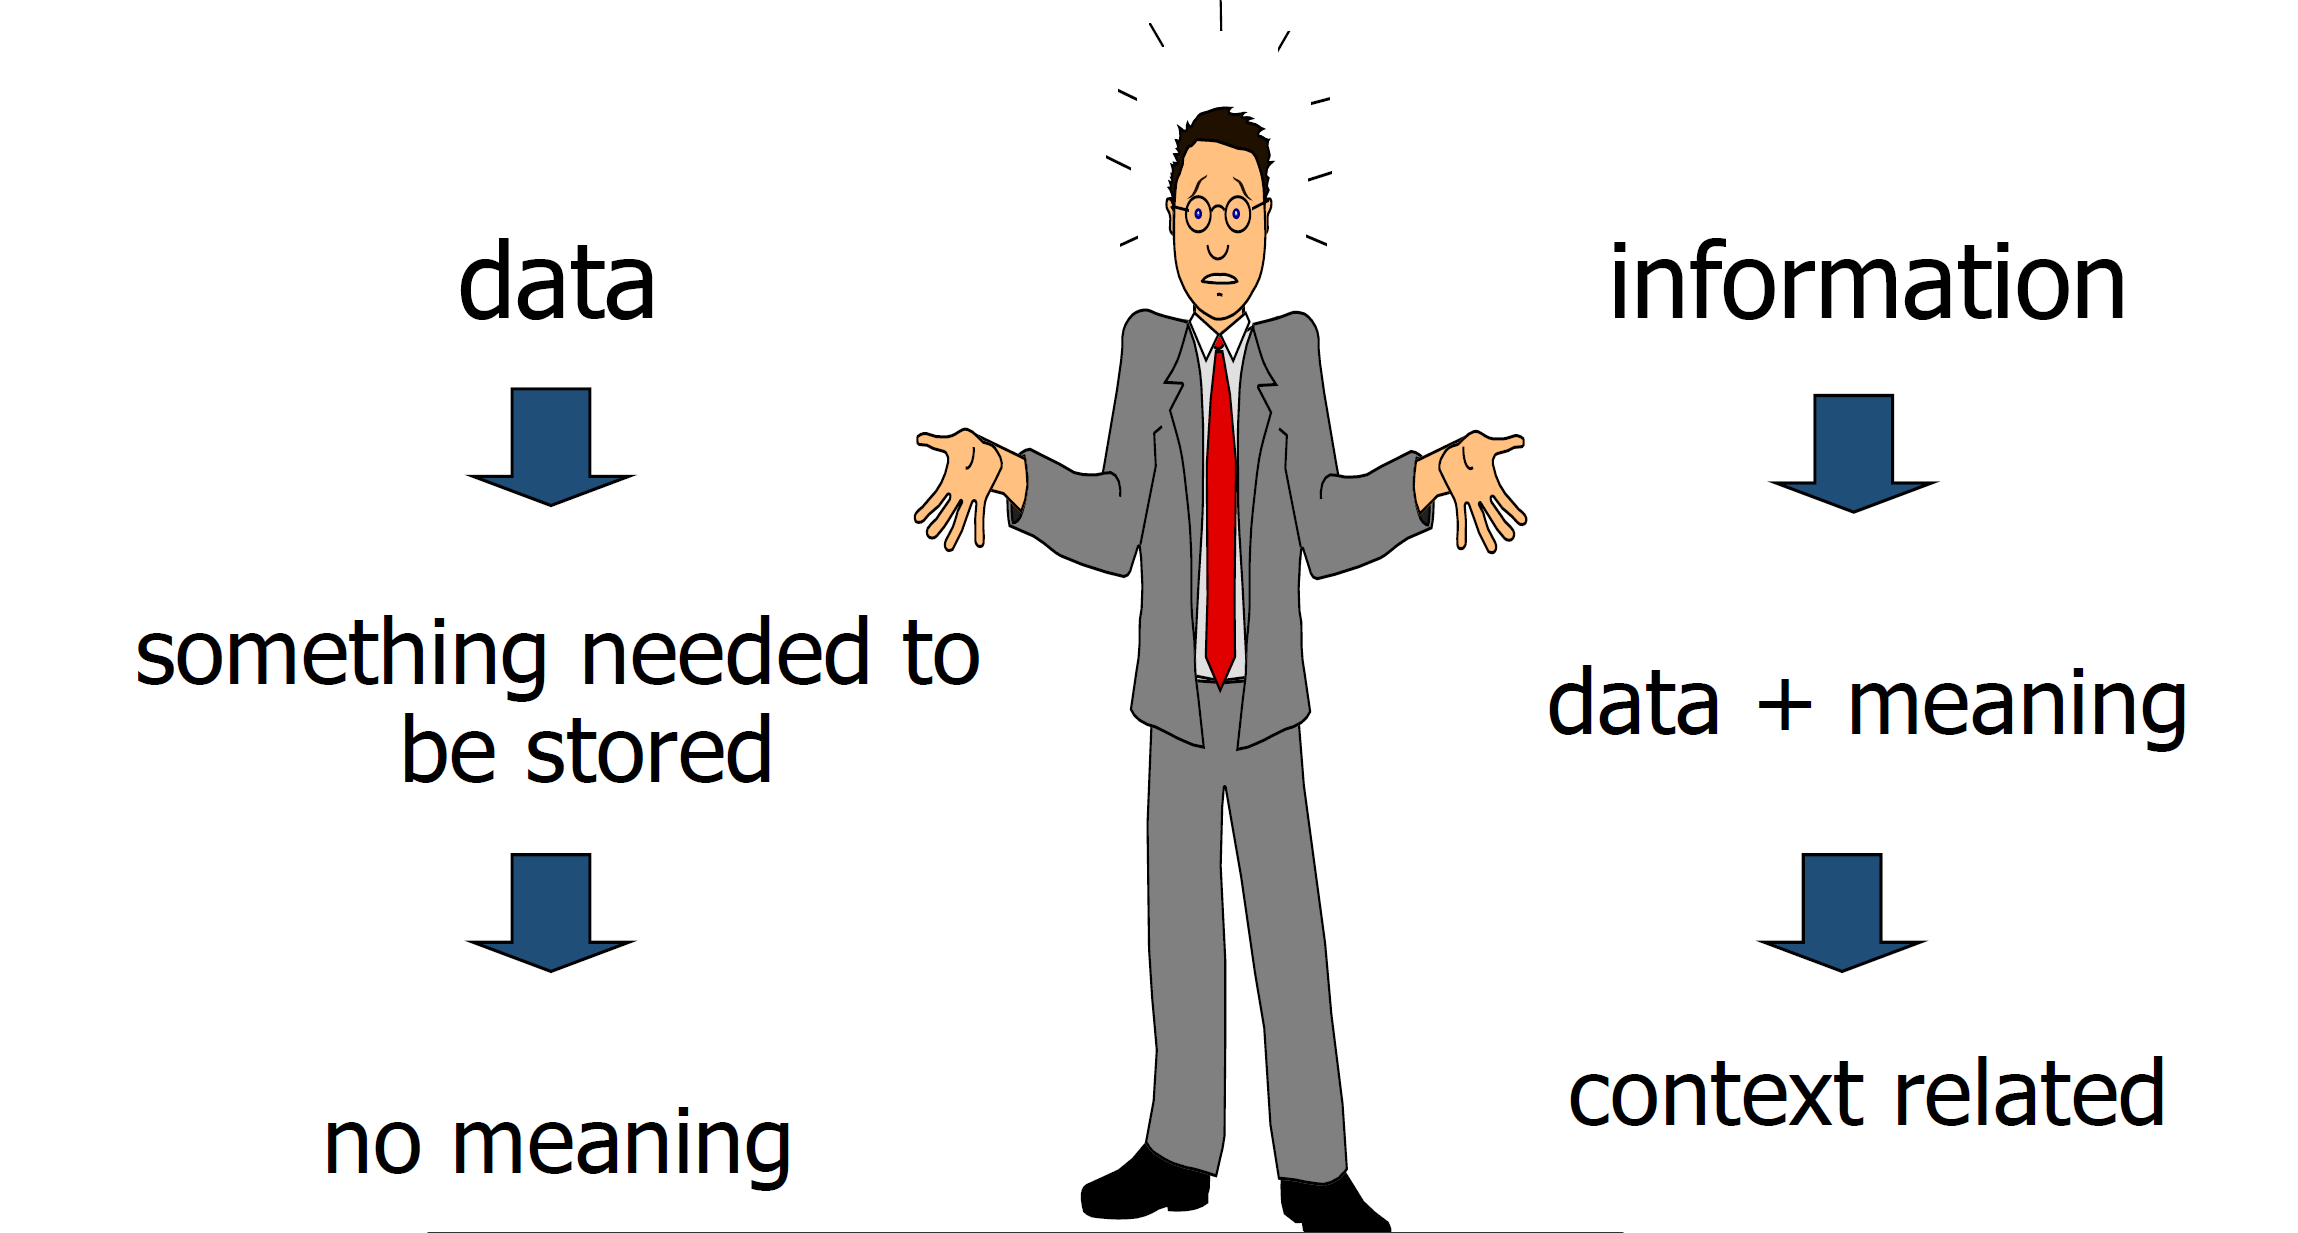
\includegraphics[width=4.5in]{img/theimportanceofinformation}%
\end{center}

Voor de ondersteuning van het management bij de bedrijfsvoering geldt dat de bedrijfsprocessen gecontroleerd moeten verlopen: zowel de invoer, verwerking en uitvoer moeten gecontroleerd (vergeleken met vooraf vastgestelde normen) en,indien nodig, bijgestuurd kunnen worden.

Opdat een organisatie goed zou functioneren, is een goed informatiebeheer noodzakelijk, aangezien de aanwezigheid van de juiste informatie op het juiste moment op de juiste plaats van doorslaggevend belang kan zijn voor de organisatie. Aangezien dus het informatiesysteem ontwikkeld moet worden in en voor de organisatie en in nauwe samenwerking met mensen uit die organisatie, is een goed inzicht in de organisatie noodzakelijk. De werkwijze moet afgestemd worden op de organisatie, de haalbaarheid van veranderingen moeten ingeschat kunnen worden, de keuze van juiste gesprekspartners in de loop van de systeemontwikkeling, en dergelijke zijn degelijke argumenten om voldoende tijd te stoppen in het leren kennen van de organisatie.

\begin{center}
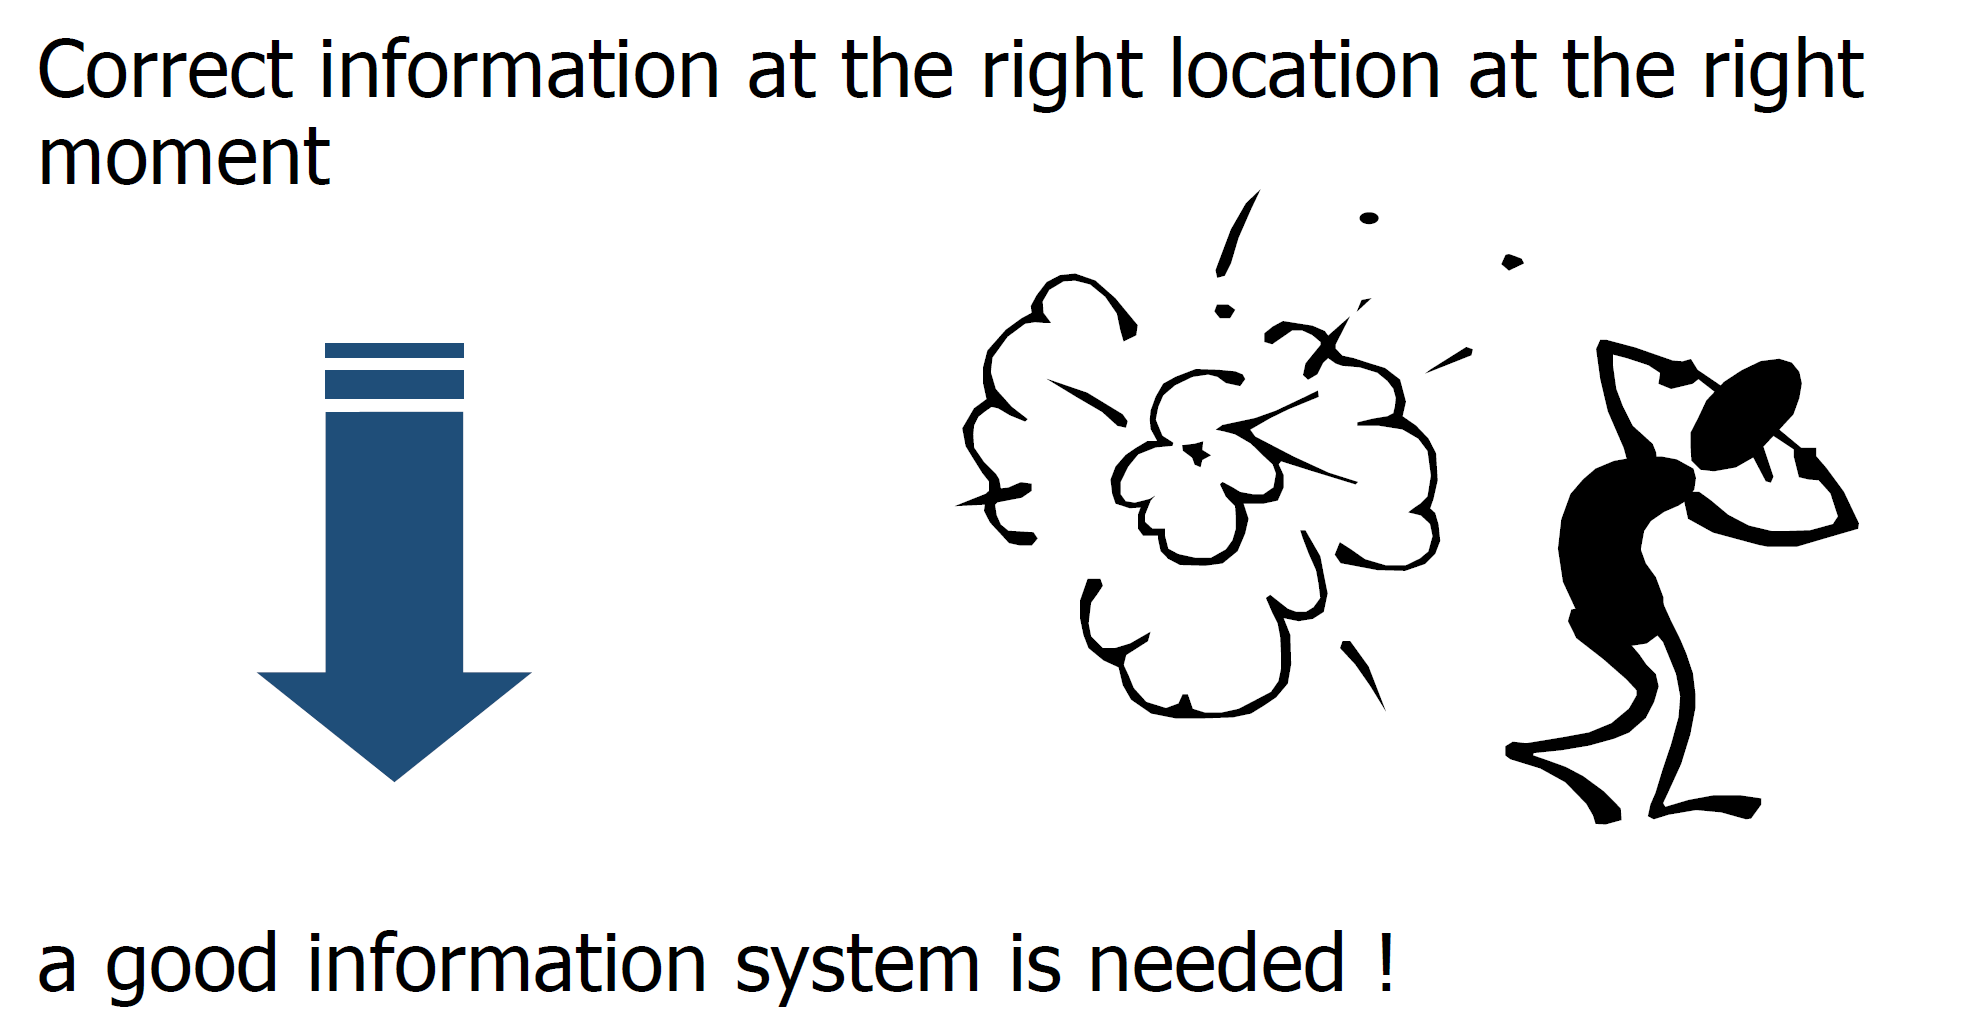
\includegraphics[width=4in]{img/theimportanceofinformation2}%
\end{center}

\subsection{Een informatiesysteem}

\subsubsection{What is an informationsystem?}

\textcolor{red}{Systeem} = een verzameling op elkaar inwerkende componenten, die volgens een bepaald plan geordend zijn, teneinde een bepaald doel te bereiken.

\textcolor{red}{\Gls{informationsystem}} = system that is responsible for collecting, managing, storing and processing of data and for providing information that is of value in forming judgments and to perform activities in the organization

\subsection{Characteristics of a System}

\begin{center}
            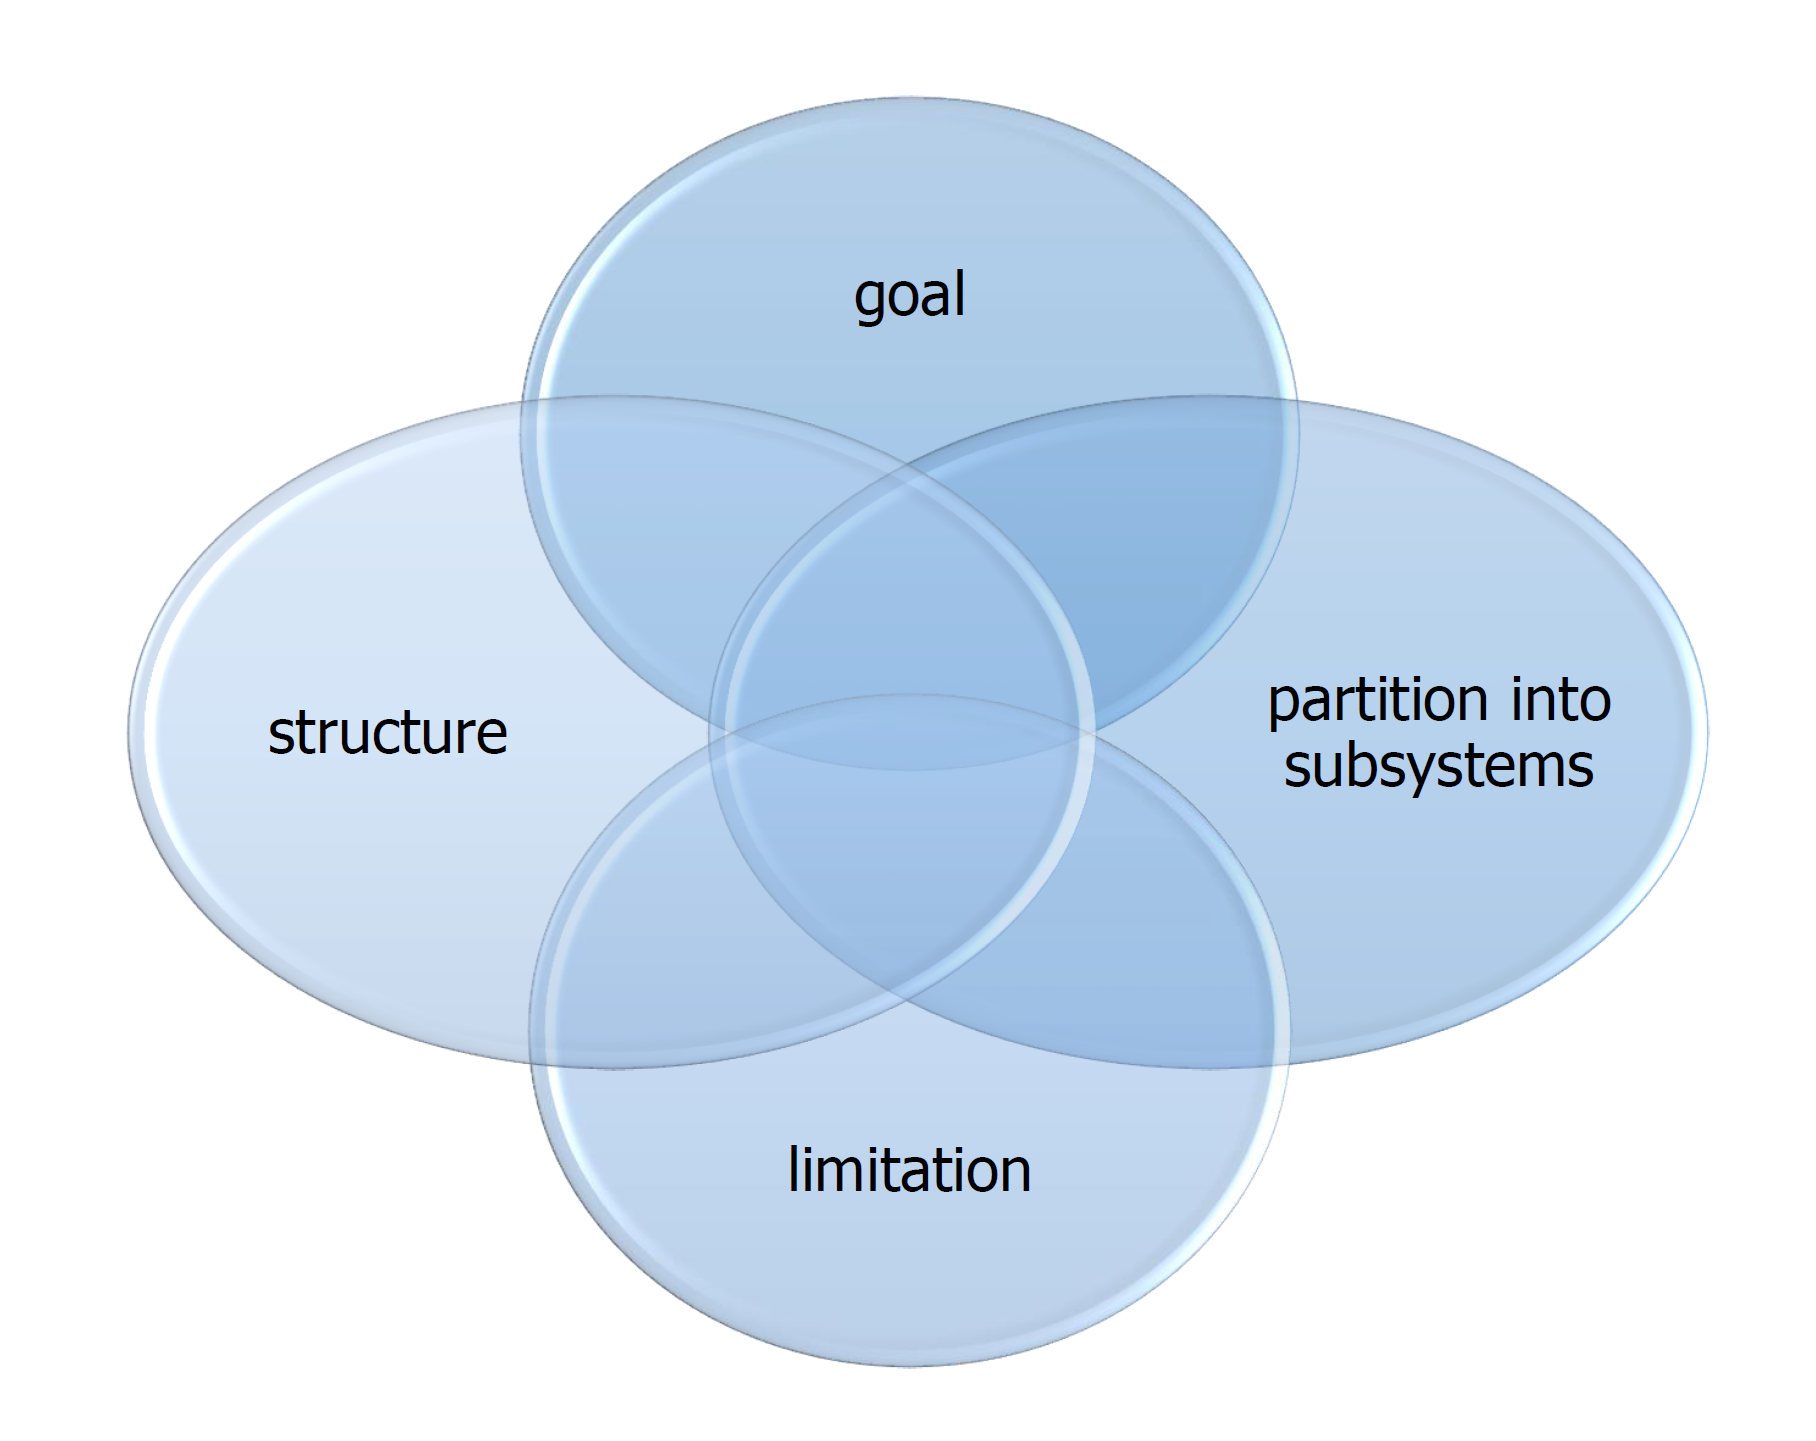
\includegraphics[width=4in]{img/osa1.PNG}
\end{center}

\subsubsection{Definitie}

Tussen die componenten bestaan een aantal relaties. Het systeem is dus een te ontwerpen eenheid, of een verzameling van functies die als geheel ontworpen zouden moeten worden.

Deze componenten voldoen aan een aantal voorwaarden, zodat voor elk element in de organisatie bepaald kan worden of het al dan niet tot deze verzameling behoort. De combinatie van de verzameling elementen die aan deze voorwaarden voldoen en de relaties die tussen deze elementen bestaan, vormt het systeem. Het geheel van die relaties vormt de structuur van dat systeem. Alles wat zich buiten deze grenzen bevindt, behoort tot de systeemomgeving.

\subsubsection{Informatiesysteem}

Een informatiesysteem is een systeem dat instaat voor het verzamelen, beheren, opslaan en verwerken van gegevens. Het is ook verantwoordelijk voor het verstrekken van informatie die van waarde is bij het vormen van oordelen en het verrichten van activiteiten in de organisatie. Het is dus een informatie verwerkend en producerend proces dat tot doel heeft in de informatiebehoeften van de business professionals te voorzien.

\subsubsection{Kenmerken}

Elk systeem voldoet aan een aantal kenmerken:

\begin{itemize}
\item Elk systeem heeft een \textbf{bepaald doel}. Deze houdt in dat een bepaalde vooraf gespecificeerde functie vervuld moet worden door het systeem. Op het niveau van de organisatie moet het systeem de doelstellingen van de organisatie ondersteunen.
\item Elk systeem \textbf{kan opgedeeld worden in een aantal deelsystemen} (dit zijn tot stand gebrachte eenheden die samen het geheel construeren), die elk hun eigen doelstellingen hebben die bovendien van betekenis zijn voor de doelstelling van het geheel. Elk deelsysteem kan ook beschouwd worden als een systeem op zich. Deze opdeling in deelsystemen gebeurt als een gefaseerde uitvoering gewenst is, of als de ontwikkeling van het gehele systeem te ingewikkeld ofte kostbaar is.
\item Elk systeem heeft een \textbf{goed gedefinieerde begrenzing}. Alles wat buiten die grenzen valt, behoort tot de systeemomgeving.
\item Elk systeem heeft een \textbf{zekere structuur}. Deze structuur wordt gevormd door het geheel van de relaties tussen de elementen van het systeem.
\end{itemize}

\newpage
\subsubsection{Eisen voor een goed systeem}

Een goed systeem moet voldoen aan de volgende voorwaarden:

\begin{center}
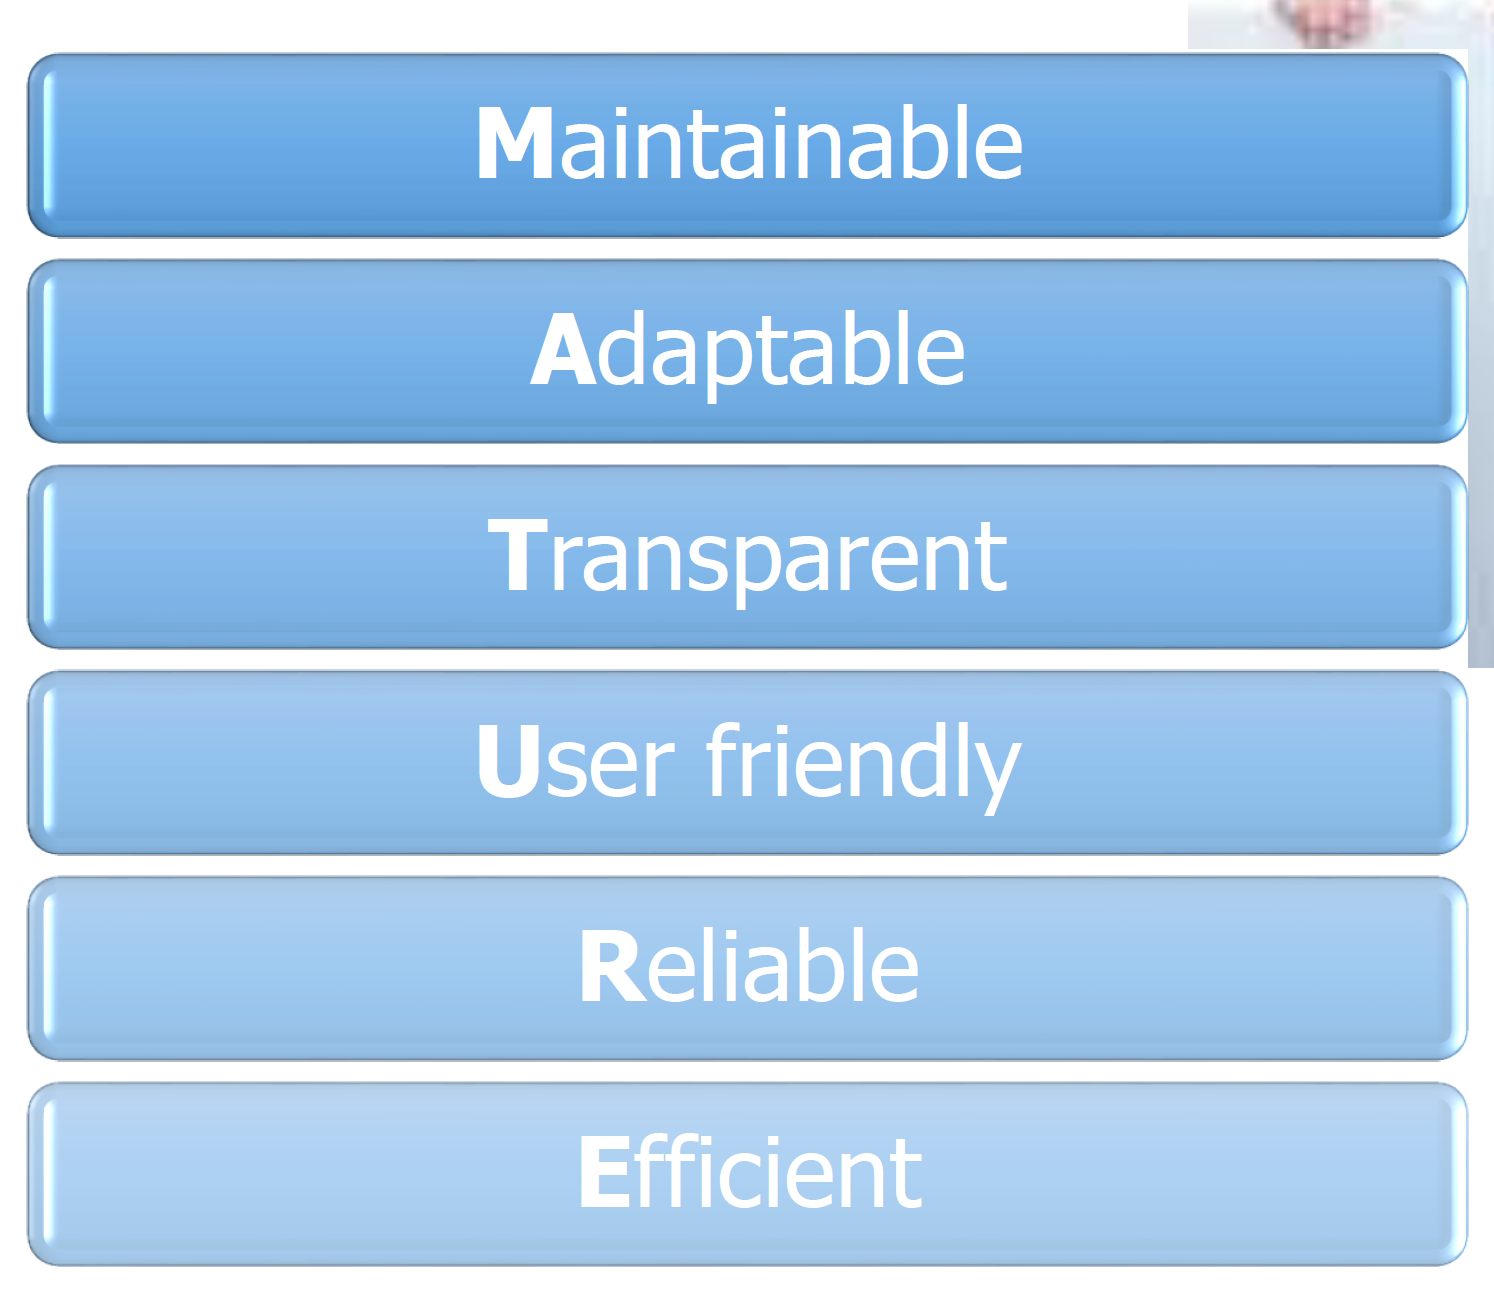
\includegraphics[width=4in]{img/requirementsforgoodsystem}%
\end{center}

\begin{itemize}
\item \textbf{Maintainable (onderhoudbaarheid):}
Het systeem moet onderhoudbaar zijn. Dit wil zeggen dat het mogelijk moet zijn fouten te verbeteren zonder nieuwe fouten te introduceren. Bovendien moet dit zo weinig mogelijk tijd en inspanning vragen. Uiteindelijk is het onderhoud een opportuniteitskost: het kost veel mensen, tijd en middelen, maar heeft als enige doel ervoor te zorgen dat het systeem blijft draaien.
\item \textbf{Adaptable (aanpasbaarheid):}
Het systeem moet ook aanpasbaar zijn. Dit wil zeggen dat de nodige aanpassingen zo vlug en eenvoudig mogelijk moeten kunnen gebeuren.
\item \textbf{Transparant}:
Het systeem moet transparant zijn. Dit wil zeggen dat de business professional alleen het eindproduct mag zien, geen technische details. Naarmate het systeem doorzichtiger wordt, zal het ook betrouwbaarder, beter onderhoudbaar en gemakkelijker aanpasbaar worden.
\item \textbf{User Friendly (gebruikersvriendelijk)}:
Het systeem moet gebruikersvriendelijk zijn. Dit wil zeggen dat het gemakkelijk leesbaar moet zijn. Het moet ook eenvoudig zijn wat betreft de door de business professional uit te voeren handelingen. Dit heeft niet alleen te maken met grafische user interfaces, maar met nog veel meer.
\item \textbf{Reliable (betrouwbaarheid):}
Het systeem moet betrouwbaar zijn. Dit wil zeggen dat het conform met de systeem specificaties moet handelen. Deze eis is van steeds groter belang, aangezien een steeds groter wordend gedeelte van de administratieve en technische processen automatisch gestuurd wordt. Een systeem kan maar betrouwbaar genoemd worden als het zowel correct als robuust (het vermogen om te blijven functioneren onder niet normale omstandigheden) is.
\item \textbf{Efficiency:}
Het systeem moet efficiënt zijn. Dit wil zeggen dat de gegevens verwerkt moeten worden tegen de laagst mogelijke kost.
\end{itemize}

\subsubsection{Modellen}

Bij het voorstellen van systemen wordt veelvuldig gebruik gemaakt van modellen. \textcolor{red}{Een model is een systeem dat een structurele gelijkenis heeft met een ander systeem}. Een model wordt \textbf{gebruikt} om informatie te krijgen over een ander systeem. Hierbij wordt gebruik gemaakt van \textbf{abstractie}. Bij het maken van abstractie worden bepaalde aspecten van het te modelleren systeem weggelaten om andere aspecten beter te laten opvallen.

\textbf{Voorbeeld.}

Een landkaart is een model voor een land en wordt gebruikt om bepaalde informatie over dat land te geven (welke steden, wat is de hoofdstad,...)- Al naargelang de bedoeling van de landkaart, zullen bepaalde dingen al dan niet getekend worden.
Zo kunnen we ook zeggen dat een informatiesysteem een model is van een deel van de organisatie (het reële systeem).

%3.
\subsection{De evolutie in systeemanalyse}

Systeemanalyse wil letterlijk zeggen: \textcolor{red}{de analyse van een systeem}. In deze context wordt bedoeld: de analyse van een informatiesysteem. Er wordt dus verwezen naar het ganse proces dat zich afspeelt vanaf het moment dat de nood aan een geautomatiseerd informatiesysteem onderkend wordt, tot het moment dat dit systeem afgeleverd wordt.

Systeemanalyse kan het best vergeleken worden met het bouwen van een woning. Het is niet omdat het huis in een bepaalde volgorde van activiteiten gebouwd wordt, dat het ook in die volgorde ontworpen wordt. De architect zal niet beginnen met het ontwerpen van de fundamenten voordat hij de rest van de woning uitgetekend heeft. Het ontwerpen van informatiesystemen kan hiermee goed vergeleken worden.

Systeemanalyse zoals dit vandaag 'gekend' is, is niet zomaar van vandaag op morgen ontstaan. Daarin heeft zich een ganse evolutie voorgedaan die hieronder beschreven wordt.

\subsubsection{Vroeger: \textquotedblleft The bad programmer\textquotedblleft }

Tot de jaren 1960 ontstonden informatiesystemen als ad hoe oplossingen voor bepaalde problemen. Men ging ongestructureerd en niet planmatig te werk. Daardoor echter kwam men tot allerlei eilandautomatiseringen: automatiseringen van verschillende problemen die niet op elkaar afgestemd waren. Dit veroorzaakte grote problemen voor het consistent houden van de gegevens, maar ook een enorme inspanning voor het onderhoud van deze systemen en hun gegevens.

Het gevolg was dus een 'spaghetti code’ met de volgende \textbf{kenmerken}:
\begin{multicols}{2}
\begin{itemize}
\item Onoverzichtelijk
\item Complex
\item Moeilijk aanpasbaar
\item Moeilijk te testen
\item Juistheid was moeilijk na te gaan
\item Onleesbaar
\item Niet onderhoudbaar
\item Niet schaalbaar
\item Moeilijk beheersbaar
\item ...
\end{itemize}
\end{multicols}

\subsubsection{Huidige problemen}

Naar aanleiding van de vroegere manier van werken, worden bedrijven nu geconfronteerd met een aantal problemen. Een uitgebreide studie werd hieromtrent uitgevoerd, aangezien men eerst de problemen moet kennen alvorens ze te kunnen oplossen. De volgende problemen werden onderkend:

\begin{itemize}
    \item de systemen voldoen niet aan de informatiebehoeften
    \item starheid van de informatiesystemen
    \item onderhoud van bestaande systemen
\end{itemize}


\subsubsubsection{systemen voldoen niet aan de informatiebehoeften}

Bij veel organisaties is men tot de conclusie gekomen dat de informatiesystemen niet voldoen aan de informatiebehoeften. Mogelijke oorzaken hiervoor zijn:

\begin{itemize}
    \item \textcolor{green}{Problemen bij het bepalen van de informatiebehoeften.}
Vooraleer een informatiesysteem gebouwd kan worden, moeten de informatiebehoeften bepaald worden. Met andere woorden: er moet bepaald worden aan welke eisen het systeem moet voldoen. Hiervoor gaat men te rade bij de business professionals en hun management. Hier doen zich een aantal problemen voor. Een tweetal zaken liggen hier aan de grondslag, er is namelijk een grote communicatiekloof tussen de ontwikkelaar (die een specialist is op het gebied van informatica, maar weinig weet over het domein dat geautomatiseerd moet worden) en de business professional (die een specialist is op zijn eigen domein, maar weinig weet over informatica en zijn mogelijkheden). Bovendien zijn de informatiebehoeften heel veranderlijk.
    \item \textcolor{green}{Gegevensvervuiling.}
Door het foutief of slordig gebruik maken van de informatiesystemen en hun gegevens, ontstaat gegevensvervuiling. Bovendien worden informatiesystemen niet altijd gebruikt voor de oplossing van het probleem waarvoor ze ontworpen werden.
    \item \textcolor{green}{Informatieverdichting.}
De business professional wordt overrompeld met massa's informatie, en dan nog meestal onder de verkeerde vorm of op het verkeerde ogenblik. De business professional heeft echter nood aan de juiste informatie onder de juiste vorm, op het juiste moment (cf. concurrentiepositie).
    \item \textcolor{green}{Slechte communicatie.}
Door een slechte communicatie tijdens de ontwikkeling van informatiesystemen, doen zich regelmatig misverstanden voor. Doordat de business professional zich verkeerd uitdrukt, ofwel doordat de systeemanalist de verkregen informatie verkeerd begrepen of geïnterpreteerd heeft. Daardoor krijgen veel business professionals de verkeerde informatie onder een verkeerde vorm, op het verkeerde moment.
\end{itemize}

\newpage

\subsubsubsection{Starheid van de informatiesystemen}

Een ander probleem dat zich voordoet bij huidige informatiesystemen, is dat ze niet flexibel aangepast kunnen worden aan de veranderende omstandigheden. Nochtans is het snel kunnen inspelen op de steeds veranderende samenleving een \textcolor{green}{kritische succesfactor (CSF)} voor het bedrijf. Bovendien biedt het flexibel kunnen aanpassen van de informatiesystemen aan de veranderende markt een competitief voordeel.

Doordat de systemen zo moeilijk aan te passen zijn (kleine wijzigingen leiden tot fundamentele herzieningen van het informatiesysteem), wordt ook dikwijls afgezien van het doorvoeren van wijzigingen.
Dit gebrek aan flexibiliteit ligt ook mede aan de basis van het gigantische onderhoud dat noodzakelijk is voor de huidige systemen.

\subsubsubsection{Onderhoud van bestaande systemen}

Het gigantische onderhoud dat nodig is voor de huidige informatiesystemen slorpt veel beschikbare resources op. Heden ten dage wordt 70 a 80 procent van de beschikbare tijd en andere resources opgeslorpt door het onderhoud van bestaande systemen. Dit leidt tot een '\textbf{maintenance boom}'. Om dit anders uit te drukken kan men ook zeggen dat ieder jaar ongeveer 1200 miljard Belgische frank besteed wordt aan onderhoud.

Uit een onderzoek van MIT blijkt dat voor iedere dollar die geïnvesteerd wordt in een nieuw project, er negen dollar zal worden uitgegeven aan onderhoud gedurende de levenscyclus van het project. Dit heeft een enorme impact op de werkomstandigheden en op de competitieve positie van het bedrijf. Er ontstaat ook een enorme backlog (achterstand) op de ontwikkeling van de nieuwe systemen: voor het starten van de ontwikkeling van nieuwe systemen moet gemiddeld 2 a 4 jaar gewacht worden, waardoor een grote achterstand ontstaat in het realiseren van nieuwe toepassingen. Dit wordt ook het \textbf{flessenhalsprobleem} genoemd (zie figuur hieronder).

%afbeelding plaatsen nog

\begin{center}
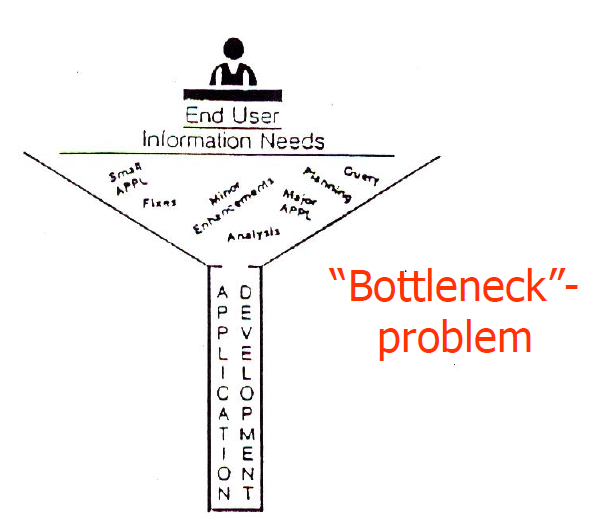
\includegraphics[width=4.4in]{img/bottleneck}%
\end{center}

In dit kader kunnen we ook de volgende uitspraak George Mc-Quilken plaatsen:
\begin{center}
\textit{\textquotedblleft Old hardware goes into museums, but old programs go into production every night\textquotedblleft}
\end{center}

Er ontstaat dus een grote kloof tussen vraag en aflevering van systemen, waarbij het ontwikkelingsproces ervaren wordt als een flessenhals. De informaticus wordt constant geconfronteerd met wijzigende vereisten en wijzigende technologieën.

\subsubsubsection{Huidige situatie}

De ontwikkeling van informatiesystemen wordt steeds belangrijker voor de totale bedrijfsplanning, aangezien de aanwezigheid van de juiste gegevens op het juiste moment op de juiste plaats doorslaggevend kan zijn voor winst of verlies voor de onderneming ('to be or not to be in the market').
Het bewustzijn ten aanzien van de invloed van informatiesystemen op de organisatie is enorm toegenomen en neemt nog altijd toe. Van informatiesystemen wordt bovendien steeds meer verwacht.

Er wordt in steeds grotere mate gebruik gemaakt van applicatie-, database- en systeemsoftware. Deze moeten dus ook op een aanvaardbare manier kunnen samenwerken.

Men heeft de problemen erkend en men is op zoek gegaan naar oplossingen voor de software crisis:

\begin{itemize}
    \item er waren grote verwachtingen van de vierde generatie talen, artificiële intelligentie, kennissystemen,... maar deze bleken de verwachtingen niet in te lossen, zodat deze niet als oplossing beschouwd kunnen worden.
    \item er werden grote inspanningen gedaan om de kwaliteit van informatiesystemen te verbeteren door gebruik te maken van gestructureerde methoden en technieken, maar deze worden weinig effectief toegepast in de bedrijven door de massa administratief werk dat met een dergelijke conversie gepaard gaat.
    \item De ontwikkeling van CASE (= Computer Aided Software Engineering) tools heeft ons een hulpmiddel gegeven bij de ontwikkeling van nieuwe systemen. Het komt tegemoet aan de nood aan verkorting van de
ontwikkelingstijd voor informatiesystemen en tevens aan het leveren van kwalitatief betere software. Let wel, CASE tools zijn een ondersteuning van de technieken, niet de vervanging ervan.
\end{itemize}

Naar aanleiding van de eerder opgesomde problemen, gaat men een inspanning doen om de ontwikkeling van informatiesystemen meer planmatig aan te pakken, in een poging om de informatieverzorging beter af te stemmen op de behoeften en noden van de organisatie. Men onderkent de nood aan een methodologie. Met andere woorden: de systeemanalyse is ontstaan.

%4.
\subsection{De software ontwikkelinglevenscyclus}

Op het moment dat begonnen werd met het onderzoeken van informatiesystemen en hoe men de huidige problemen kon verhelpen, is men tot de conclusie gekomen dat ook software een soort levenscyclus (software development lifecycle) heeft. Deze start bij de geboorte van het systeem. Dit is de ontdekking van een probleem dat geautomatiseerd zou moeten worden, een opportuniteit om de werking van de organisatie te verbeteren. Daarna worden een aantal fasen doorlopen. Op een bepaald moment wordt deze cyclus al dan niet beëindigd.
Tijdens elke fase worden een aantal stappen doorlopen, een aantal mijlpaalproducten voortgebracht.

Ook in de visie op deze levenscyclus heeft zich een ganse evolutie voorgedaan:

\subsubsection{De klassieke levenscyclus}

De oudste visie op de software ontwikkelingslevenscyclus is de klassieke visie. Hierin worden alle fasen sequentieel doorlopen, waarbij de uitvoer van de vorige fase de invoer wordt voor de volgende fase. De 'geboorte' van het systeem is de aanvraag door de business professional (User Request), waarin een vraag naar automatisering gesteld wordt. De 'dood' van het systeem is het moment dat het systeem afgeleverd wordt aan de business professional. Het systeem sterft als het ware, omdat men ervan overtuigd was, dat na het afleveren van het systeem de informaticus zich er niets meer moest van aantrekken.

%afbeelding plaatsen nog

\begin{center}
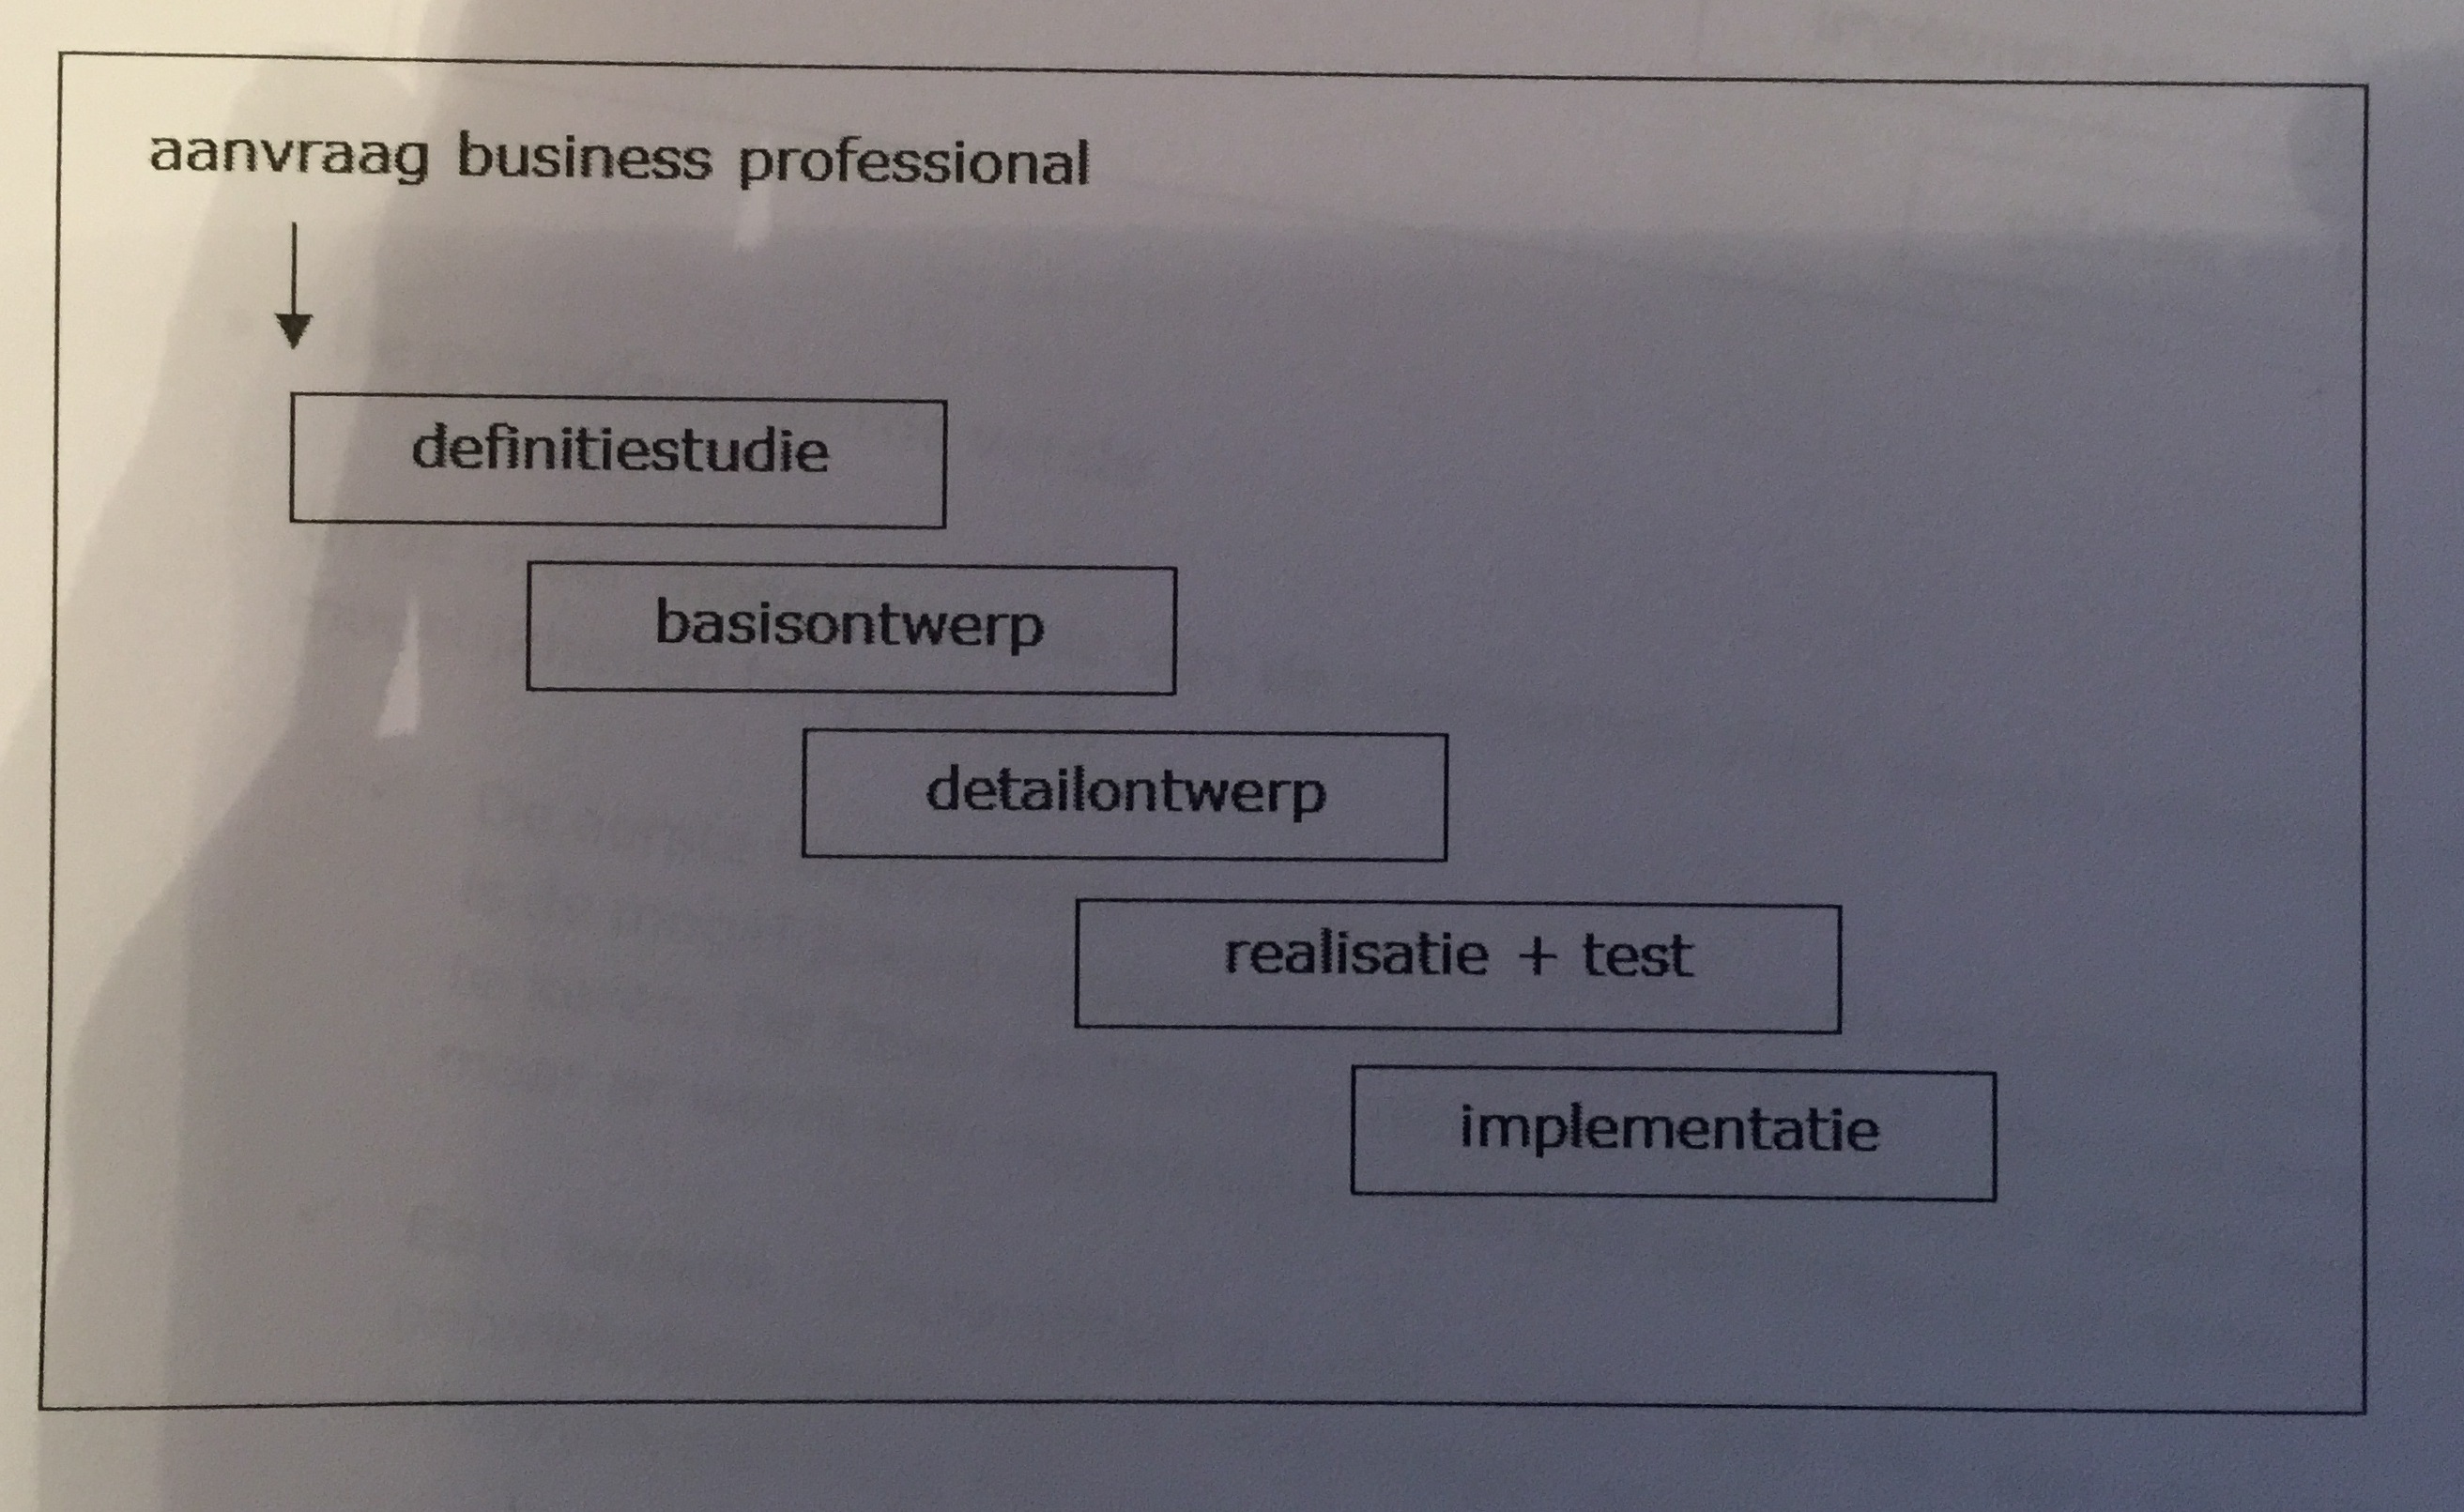
\includegraphics[width=4in]{img/IMG_3586}%
\end{center}

\subsubsection{De gestructureerde visie}

De voorgaande visie ging uit van de sterfelijkheid van de software. Heel snel echter ging men beseffen dat de zorg voor een informatiesysteem niet eindigt bij het afgeven aan de business professional. Meestal ondervindt men op het moment van afleveren nog een heleboel problemen die ook opgelost moeten worden, zoals fouten die verbeterd moeten worden, aanpassingen in de gebruikersbehoeften en aanpassingen in de technologie. Daarom heeft men er in de gestructureerde visie nog een extra fase gebruik en beheer (eternal life) aan toegevoegd, waarin in het onderhoud van het systeem voorzien wordt.

%afbeelding plaatsen nog

\begin{center}
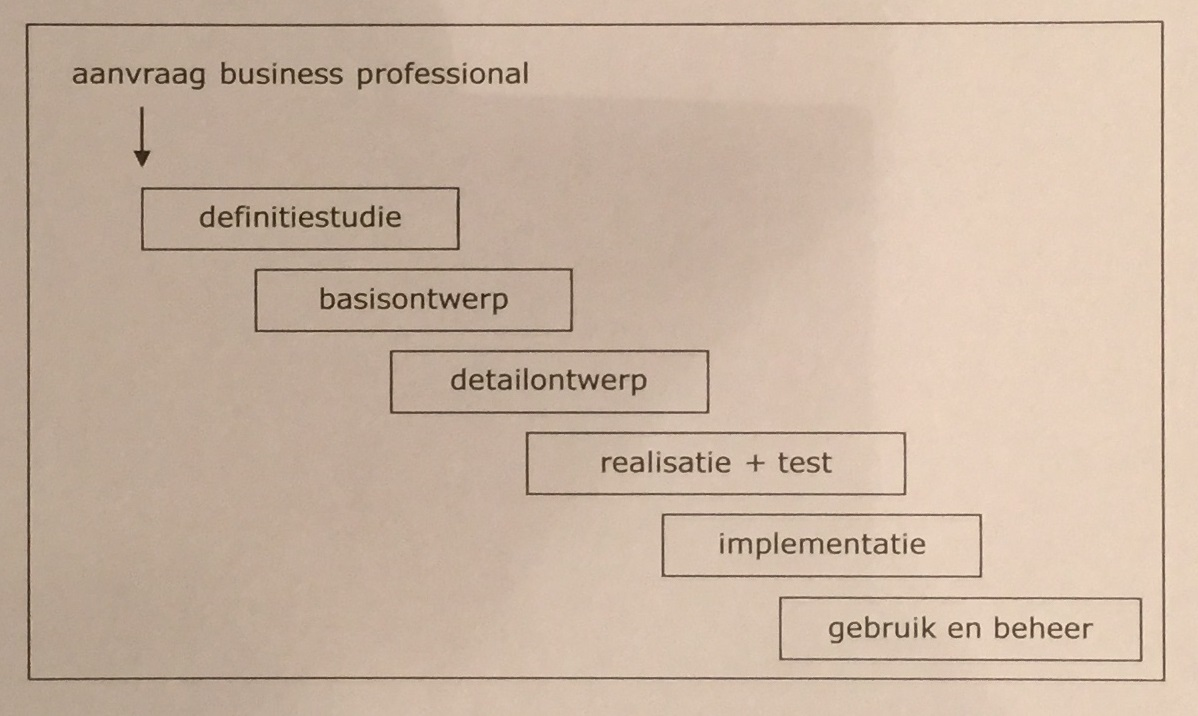
\includegraphics[width=4in]{img/IMG_3584}%
\end{center}
\newpage
\subsubsection{De gemoderniseerde visie}

In de meer moderne versie van de voorgaande visie, werden enkel een drietal mogelijkheden toegevoegd:

\begin{itemize}
    \item De eerste toegevoegde mogelijkheid is die om iteratief te werken. Hierbij is de mogelijkheid ingelast om, indien nodig, één of meerdere fasen terug te keren. De fasen worden dus niet meer netjes achter elkaar geplaatst, maar er wordt een mogelijkheid voorzien om terug te springen.
    \item Een tweede nieuwigheid is een nulde fase die aan de software ontwikkelingslevenscyclus toegevoegd werd, namelijk de strategische informatieplanning. Deze fase is er gekomen door:
        \begin{itemize}
        \item de steeds groter wordende behoefte aan goede en tijdige informatie,
        \item de steeds toenemende integratie,
        \item de steeds groter wordende invloed van automatisering op het 
        functioneren van de ganse organisatie,
        \item organisatorische veranderingen,
        \item de steeds toenemende mogelijkheden.
        \end{itemize}
    \item Een derde toevoeging is de mogelijkheid tot reverse engineering van bestaande systemen, zodat de oude systemen aangepast kunnen worden tot een vernieuwde 'propere' versie, zonder dat opnieuw van nul gestart moet worden. Een sterk punt hierbij is dat men hoopt dat deze stap automatisch zal kunnen gebeuren, zodat het onderhoud van bestaande systemen op die manier verminderd zal kunnen worden:
\end{itemize}

Het doel van reverse engineering is zesvoudig:

\begin{itemize}
    \item de complexiteit van het systeem onder controle krijgen,
    \item alternatieve zienswijzen creëren,
    \item zoveel mogelijk verloren informatie terugwinnen,
    \item nevenverschijnselen die in bestaande software geslopen zijn, trachten te achterhalen,
    \item ervoor zorgen dat voorstellingen gecreëerd worden met een hoger niveau van abstractie,
    \item opnieuw bruikbaar maken van bepaalde softwarecomponenten uit reeds bestaande programma's (dit wordt ook legacy-software genoemd) en de bestaande software ook integreren in het nieuwe systeem
\end{itemize}

%afbeelding nog plaatsen

\begin{center}
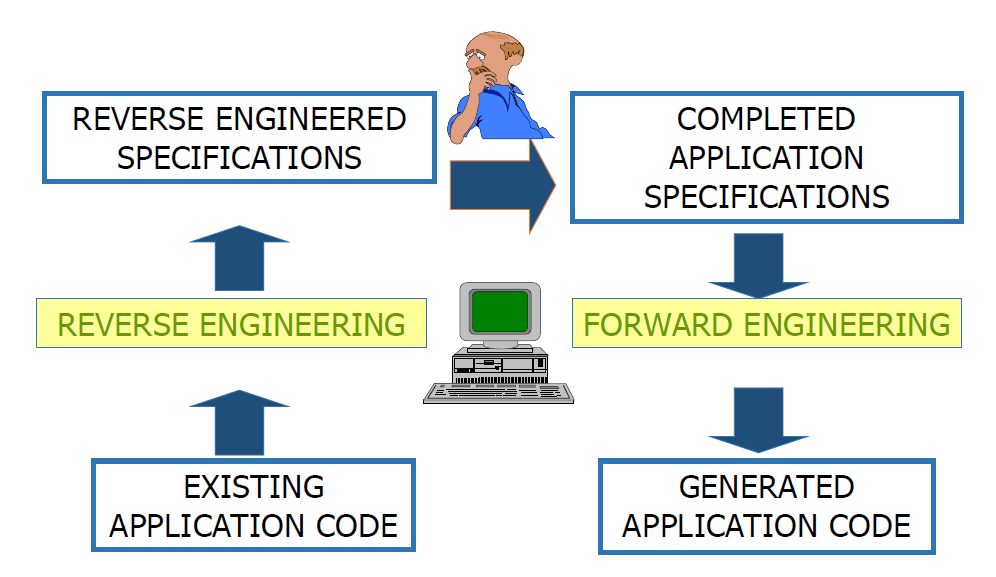
\includegraphics[width=4in]{img/reverseengineering}%
\end{center}

Reverse Engineering:
\textcolor{red}{het uit elkaar rafelen van een stuk oude code, om op deze manier achter de beginspecificaties van het systeem en/of de design specificaties te komen. Het resultaat dat men aldus bekomt, is een abstracte representatie van het systeem.}

Forward Engineering: \textcolor{red}{het top-down ontwikkelen van systemen, waarbij men de opeenvolgende fasen van de ontwikkelingslevenscyclus doorloopt.}

Re-engineering: \textcolor{red}{het volledige proces van reverse en forward engineering}


\subsubsection{De object-georiënteerde visie}

Bij de voorgaande visies doen zich een aantal problemen voor, namelijk :

\begin{itemize}
    \item Alles is gebaseerd op gebruikersbehoeften, die in wezen heel veranderlijk zijn. Er is dus geen stabiele basis als vertrekpunt. Daardoor moeten nog te dikwijls veranderingen doorgevoerd worden op de kern van het informatiesysteem. Dit vraagt nog teveel onderhoud.
    \item Het ontwerp van het informatiesysteem gebeurt volledig top-down. Dit levert problemen omdat men al te vroeg tijdens de systeemontwikkeling belangrijke beslissingen moet nemen. Daardoor worden al te vroeg teveel beperkingen opgelegd. Let wel, top-down is wel een goede werkwijze voor navigatie en documentatie.
\end{itemize}

Een oplossing voor deze problemen, is deze laatste visie, nl. \textbf{de model driven life cycle}. Bij deze visie vertrekt men niet meer van de gebruikersbehoeften maar van de stabiele kern van de organisatie, namelijk het bedrijfsmodel ('the business model'). Hierin wordt de werkelijkheid van de organisatie gemodelleerd, met alle objecten die het bedrijf en de werking ervan bepalen en de relaties die tussen deze objecten bestaan. Met andere woorden, het informatiemodel (bedrijfsmodel - business model). Dit vertrekpunt is meer stabiel, aangezien enkel veranderingen in de bedrijfsvoering aanpassingen kunnen vereisen in deze kern, en deze komen slechts zelden voor. Pas als deze kern volledig opgebouwd is, wordt daar rond een nieuwe laag gebouwd waarin de gebruikersbehoeften voldaan worden. Deze bovenste laag is heel flexibel aanpasbaar aan de veranderende gebruikersbehoeften. Daarom wordt deze benadering ook een middle-out benadering genoemd: er wordt niet top-down, noch bottom-up gewerkt, maar men vertrekt van de stabiele kern en gaat zo naar buiten toe.

Ook deze objectgerichte systeemanalyse heeft haar invloeden die een eind in de tijd teruggaan. De reden waarom ze slechts een aantal jaren geleden echt doorgebroken is, is omdat de benodigde technologie eerder nog niet voorhanden was. Zoals de figuur laat zien, was ze onderhevig aan verschillende invloeden.

\textbf{object-gericht systeem of het multiple-layer model}

Een objectgericht systeem bestaat uit een aantal objecten die gecreëerd worden, met elkaar communiceren en weer vernietigd worden. Dit alles wordt al dan niet veroorzaakt door impulsen van buitenaf.

%afbeelding nog plaatsen

\begin{center}
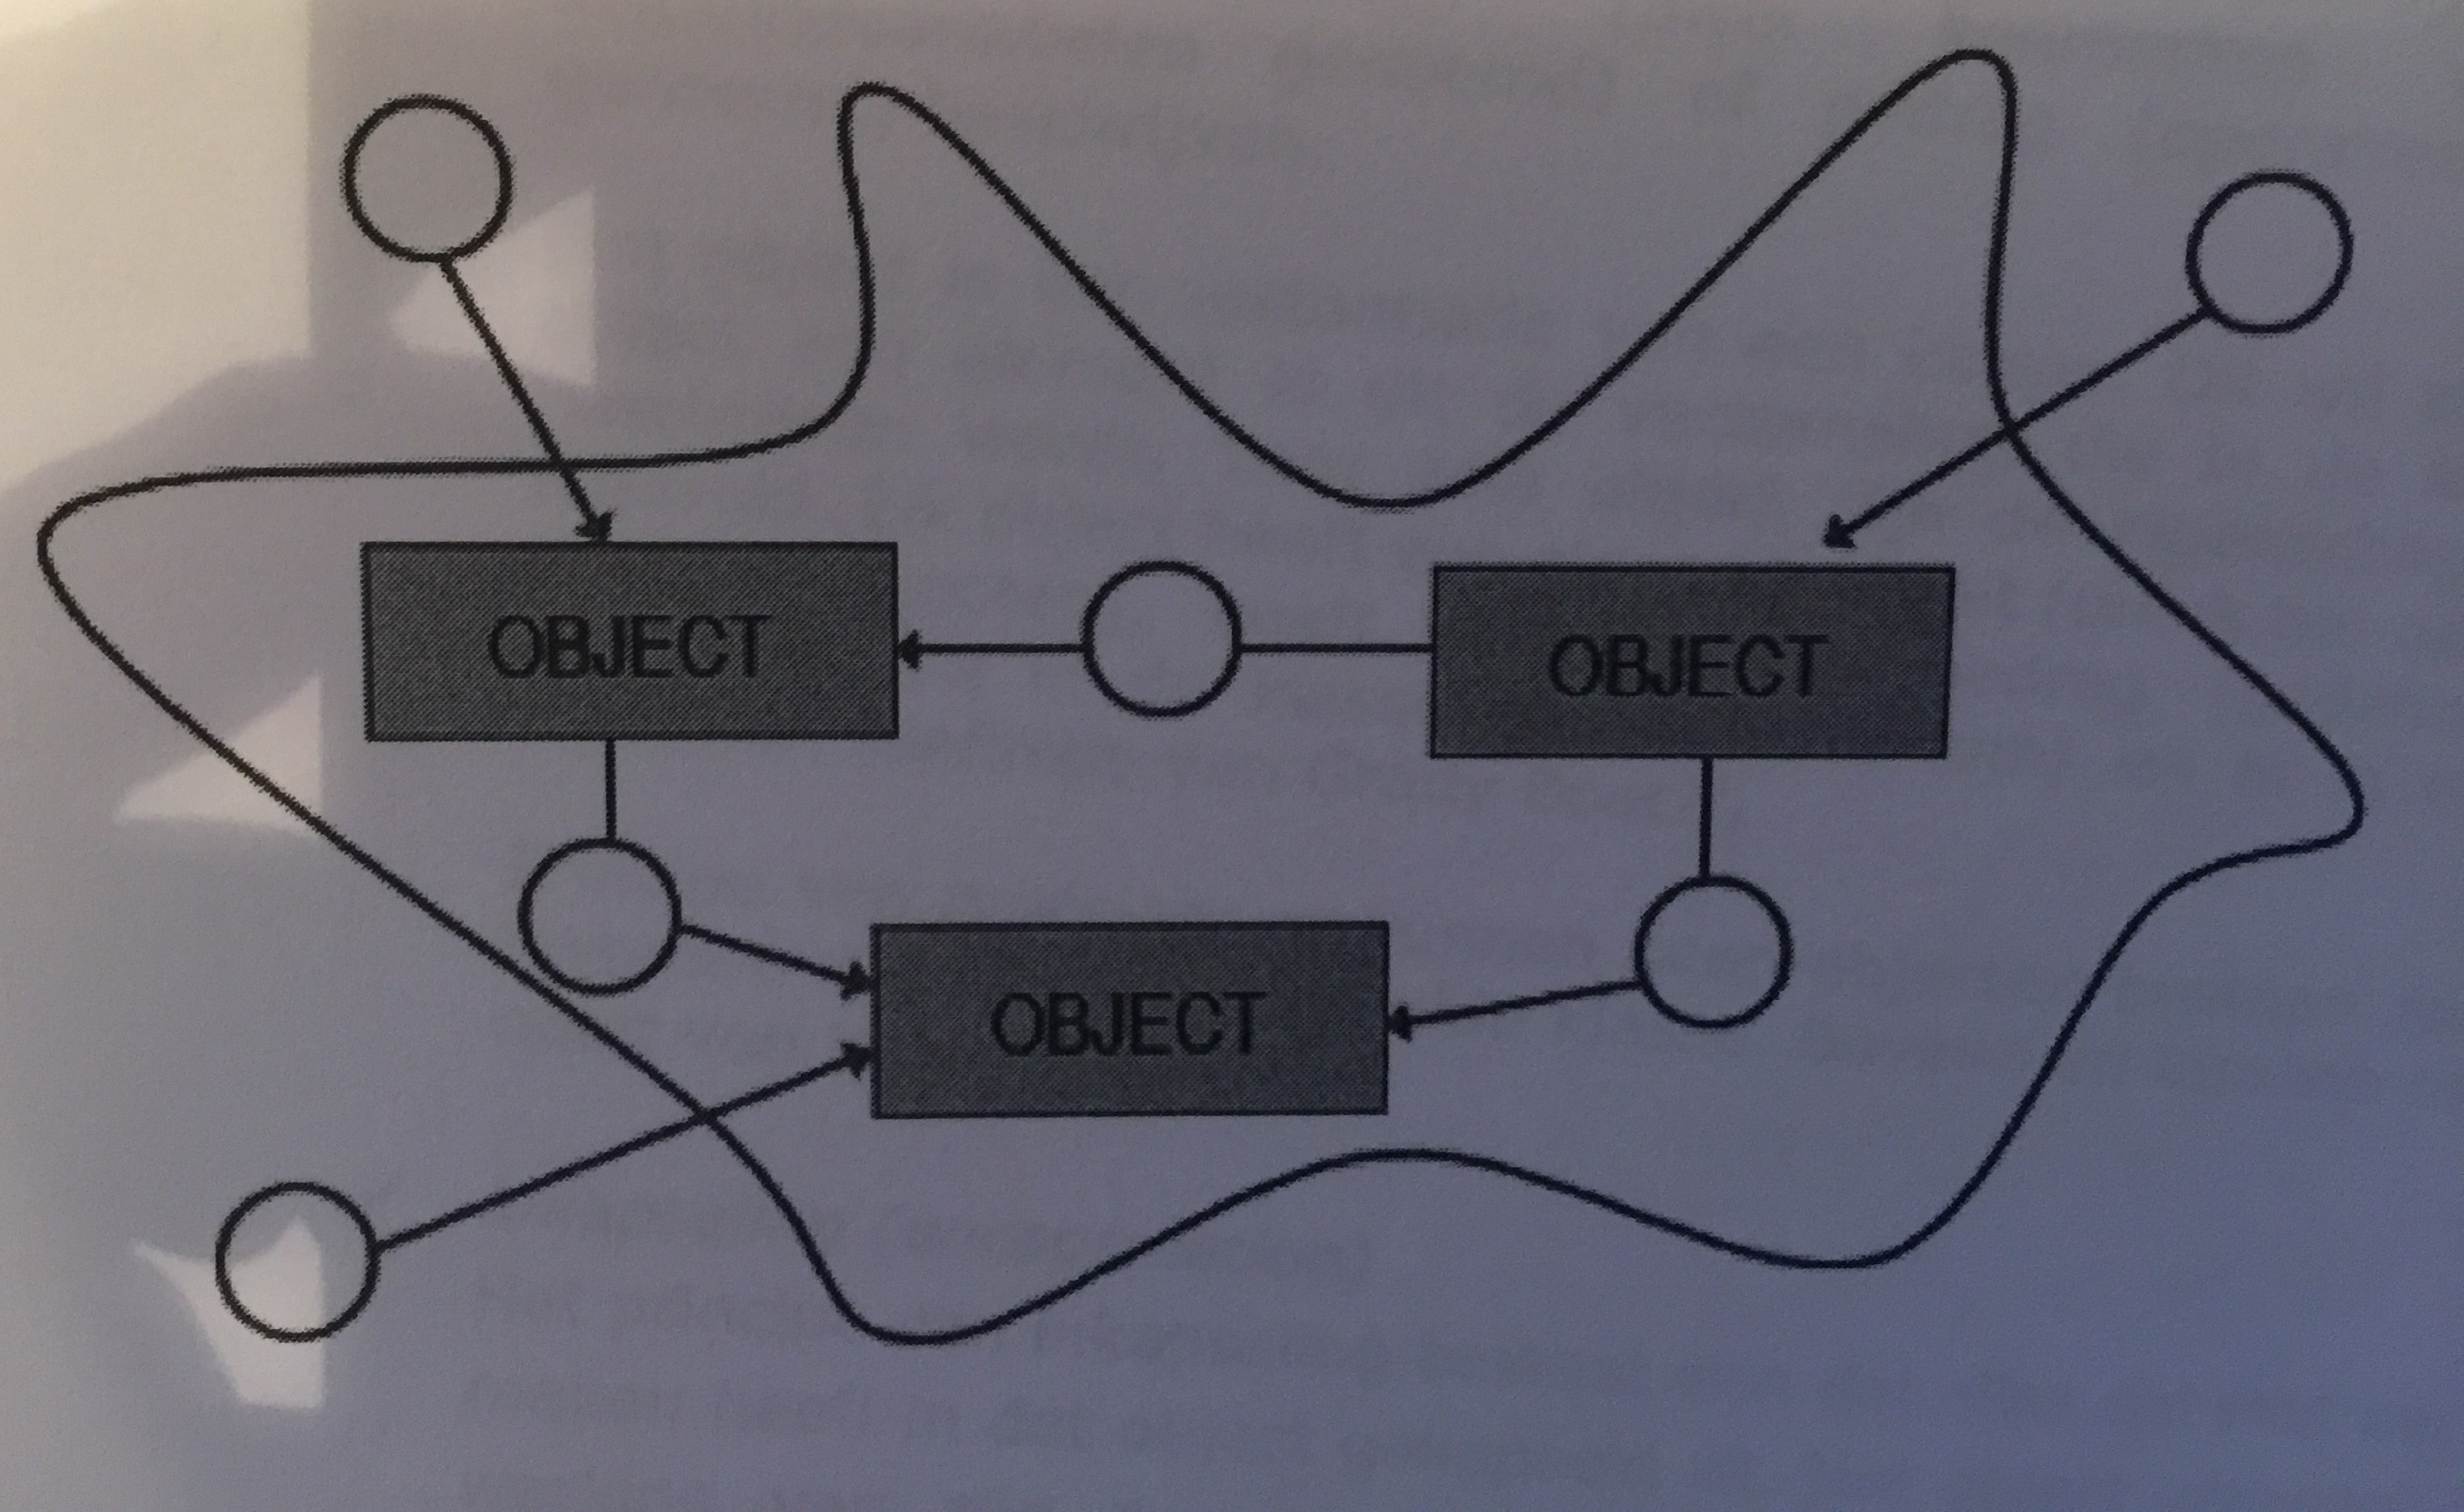
\includegraphics[width=4in]{img/IMG_3583}%
\end{center}

Alle communicatie tussen objecten onderling of tussen objecten en de systeemomgeving, gebeurt in de vorm van berichten. Er kan dus gezegd worden dat een objectgericht systeem voldoet aan de eisen van maximale cohesie (inkapseling van de objecten: alles wat met het object te maken heeft zit in het object) en minimale koppeling (de enige vorm van koppeling gebeurt via berichten en dit is de minst mogelijke koppeling die er bestaat). Vandaar dat ook gezegd kan worden dat goed ontworpen objectgerichte systemen de best onderhoudbare systemen zijn, die bovendien ook het best scoren op de andere eisen voor een goed systeem (zie eerder).

Als het systeem ontworpen wordt, moet rekening gehouden worden met het multiple-layer model (soms ook het ajuinmodel genoemd). Dit bestaat erin dat de objecten binnen het systeem zodanig ingekapseld zitten in een bepaalde laag dat altijd ervan uit gegaan kan worden dat als een bepaalde laag veranderd moet worden, dit enkel invloed heeft op objecten in deze laag of in een laag erbuiten en dus nooit effect heeft op objecten in een meer naar binnen gesitueerde laag.

Dit idee werd reeds gepubliceerd door Michael Jackson in de jaren 1970, maar heeft nooit eerder doorgang gekend wegens de lange wachttijden die het teweeg bracht. Het duurde te lang vooraleer alle lagen ontworpen waren zodat het systeem in productie gebracht kon worden.

Met de huidige objectgerichte technieken echter wordt dit opgelost door middel van time-boxing. Dit is een manier waarop componentsgewijs gewerkt wordt: de taart wordt verdeeld in een aantal stukken (time-boxes) zodat de 3x3 regel gerealiseerd kan worden: elke time-box moet gerealiseerd kunnen worden door 3 personen in een periode van 3 maand. Hierbij is natuurlijk wel vereist dat het bedrijfsmodel grondig uitgewerkt is, en dat er voldoende controle is om de consistentie en samenhang van het geheel te waarborgen.
\newpage

\textbf{basisconcepten van object-oriëntatie}

\begin{itemize}
    \item klasse vs object
    
Een klasse geeft een gedetailleerde beschrijving van een aantal dingen met dezelfde eigenschappen en die hetzelfde gedrag vertonen. Deze eigenschappen kunnen zowel kenmerken (attributen of instantievariabelen genoemd) of gedrag (operaties of methodes genoemd) beschrijven.

Een object is een instantiatie van een klasse. Dit wil zeggen dat een object een element is uit de verzameling die in de klassendefinitie beschreven wordt. Voor zo'n object zijn de eigenschappen concreet ingevuld. Elk object heeft een eigen identiteit (uniek ten opzichte van de andere objecten), heeft een bepaald gedrag (gedefinieerd in de methodes die in de klasse gedefinieerd zijn) en is in een bepaalde toestand, (definitie van Grady Booch)

Principe van typering: er kunnen geen objecten bestaan zonder dat ze instantie zijn van een bepaalde klasse. Bovendien kunnen objecten ook nooit van type veranderen.
    \item inkapseling (encapsulation)
    
    
Het principe van inkapseling bestaat erin dat alles dat met een object te maken heeft in dat object gekapseld zit. Het object verbergt de interne werking van zijn operaties voor de buitenwereld en voor andere objecten. Dit heeft als gevolg dat aanpassingen aan één object meestal geen gevolgen hebben voor andere objecten.

Voorbeeld. 

je moet niet de werking van de afstandsbediening van de TV kennen om deze te kunnen gebruiken. Je hoeft niet te weten op welke manier de signalen doorgezonden worden om naar een andere zender te kunnen kijken.
    \item informatieverberging (Information hiding)
    
Dank zij het principe van inkapseling kan dit principe van informatie verberging gerealiseerd worden. Het principe houdt in dat zo weinig mogelijk over het object bekend gemaakt wordt. De attributen en de operaties worden zo privaat mogelijk gedefinieerd, enkel publiek als daar een goede reden voor is. Enkel de interface van het object is gekend naar buiten toe...
Het voordeel hierbij is dat als intern iets verandert, zonder de interface te veranderen, de buitenwereld dit zelfs niet moet weten.
    \item polymorfie
    
Bij het principe van polymorfie bepaalt het ontvangend object welke methodedefinitie uitgevoerd wordt. De zender hoeft dus niet te weten naar welk soort object zijn boodschap verstuurd wordt, de ontvanger weet exact welk soort object hij is en dus welke methodedefinitie uitgevoerd moet worden.

Voorbeeld. 

De operatie openen in de klasse Bankrekening heeft een totaal andere betekenis dan de operatie met dezelfde naam in de klasse Venster
\newpage
    \item generalisatie (overerving)
    
Bij generalisatie gaat het om de classificatie van klassen van dezelfde soort. De mogelijkheid bestaat hierbij om een hiërarchische structuur te verwezenlijken tussen de klassen door aan te geven dat een bepaalde klasse overerft van een andere. Als dit het geval is, dan erft de ene klasse alle eigenschappen van de andere over en kan daar nog iets specifiek aan toevoegen.

Let op bij het toepassen van dit principe, dat het niet te ver doorgedreven wordt: het kan namelijk een extra moeilijkheidsgraad toevoegen aan het principe van typering: een object gegenereerd uit een subtype, kan nooit van subtype veranderen.

Voorbeeld. 

Een kamer in een hotel kan bepaalde functies vervullen: slaapkamer, vergaderruimte, enz. Om hiervan subtypes te maken, zou niet goed zijn aangezien een kamer wel van functie kan veranderen: bijvoorbeeld in het hoogseizoen kan van een vergaderruimte één of meerdere slaapkamers gemaakt worden.

In dit geval kan je beter een associatie leggen tussen kamer en het gebruik ervan, een soort van contractsgewijs verband.
    \item package
    
Een extra mogelijkheid om diagrammen uit te breiden is door bepaalde klassen die samenwerken om aan een bepaalde verantwoordelijkheid te voldoen samen te nemen in een groep. Er moet wel voldaan zijn aan de beperking dat een element slechts maximaal tot één package kan behoren. Er mogen dus met andere woorden geen overlappingen zijn tussen packages.
Verbanden tussen klassen uit verschillende packages duiden op dependency relaties. Om te verwijzen naar een klasse uit een ander package, gebruiken we de notatie

\begin{center} \textit{naamPackage:: naam Klasse} \end{center}
      \item notities
      
Indien een onderdeel van een diagram niet ondubbelzinnig of zichzelf verklarend is, kan met behulp van notities als het ware "gele plakbriefjes" op het diagram gekleefd worden waardoor een verklarend woordje toegevoegd wordt.
      \item dependency
      
Als er verbanden bestaan tussen modeleiementen uit verschillende packages, dan ontstaat er een dependency (afhankelijkheids-) relatie tussen beide packages. Dit betekent dat een bepaald modelelement een ander modelelement nodig heeft om goed te kunnen functioneren.

Om te verwijzen naar een klasse uit en ander package, wordt de dubbele punt notatie gebruikt.

\begin{center} \textit{naamPackage: :naamKlasse}\end{center}
\newpage
      \item stereotype
      
UML kan uitgebreid worden of aangepast aan een bepaalde manier van werken binnen een organisatie. Een stereotype is een modelelement in UML waardoor de taal uitgebreid en aangepast kan worden. Het concept wordt veel toegepast, aangezien het toelaat om eigen "typen" elementen met specifieke betekenis te maken. Met dit concept wordt een nieuw soort modelelement gedefinieerd op basis van een bestaand modelelement, maar dan met een paar extra betekenissen die het origineel niet heeft.

\textit{Generalization}

Voorbeeld. Om aan te duiden uit welke ontwikkelingslaag het element afkomstig is:

\begin{center} \textit{«bedrijfsmodel» , «user interface», enz.}\end{center}

\end{itemize}

%5.
\subsection{Beknopte beschrijving van de verschillende fasen}

Voor iedere fase geldt dat eerst aan een aantal voorwaarden voldaan moet zijn, dan worden een aantal activiteiten uitgevoerd. Aldus wordt een resultaat bekomen dat geëvalueerd wordt. Na de evaluatie van het resultaat wordt een beslissing genomen: ofwel een aantal activiteiten herhalen, ofwel doorgaan naar de volgende fase, ofwel stoppen met de systeemontwikkeling. Het grote voordeel is dat in elke fase een checklist gegeven wordt van uit te voeren acties en op te leveren mijlpaalproducten.

De resultaten van de vorige fase worden doorgegeven en gebruikt als invoer voor de volgende fase. Vandaar het belang van de evaluatie van het resultaat.

Voordelen van de opdeling in fasen zijn:

\begin{itemize}
    \item de mogelijkheid tot periodieke controle (voordeel voor de projectmanager, want voor elk van de fasen worden een aantal producten ontwikkeld die apart opgevolgd kunnen worden),
    \item het verkrijgen van een efficiënt instrument ter controle van de voortgang van de systeemontwikkeling (voordeel voor het management en de business professionals, want ze kunnen een periodieke controle uitvoeren om te zien of het systeem nog steeds aan de gestelde eisen en specificaties voldoet, teneinde de mogelijkheid te hebben tijdig te kunnen bijsturen),
    \item het verkrijgen van materiaal voor de systeemdocumentatie (mijlpaalproducten die in elke fase gecreëerd worden).
\end{itemize}
\newpage
\subsubsection{Strategische informatieplanning}

Tijdens de Strategische Informatieplanning wordt een voorstudie gemaakt, waarbij het de bedoeling is een zicht te krijgen op het bedrijf en zijn activiteiten. Er wordt een informatieplan gemaakt voor de organisatie op hoog niveau. Dit zowel op middellange als lange termijn. De te ontwikkelen systemen worden afgebakend en de prioriteiten worden vastgelegd.

Typisch voor deze fase is dat gebruik gemaakt wordt van matrices om verbanden tussen objecten van de organisatie in beeld te brengen. De techniek die hiervoor gebruikt wordt is de \textbf{Business System Planning (BSP)} of de \textbf{Information Systems Study (ISS).}

Om een beter inzicht te krijgen in de organisatiestructuur, kan gebruik gemaakt worden van organisatiestructuur schema's, die een inzicht geven in de structuur van de hiërarchische verhoudingen, en functiediagrammen, die aantonen hoe de deeltaken en beslissingsbevoegdheden over de functies of personen die samen een functie uitoefenen verdeeld zijn. Belangrijk hier zijn de bedrijfsdoelstellingen, de strategische uitgangspunten, de \textbf{Critical Success Factors (CSF)}.

\subsubsection{Analyse en logisch ontwerp}

Tijdens de Analyse wordt een snelle evaluatie gemaakt van wat de business professionals willen en de mogelijkheid en de rentabiliteit van een automatiseringsproject ten aanzien van een bepaald gedeelte van de gegevensverwerking. De te ontwikkelen systemen worden duidelijk afgebakend en de prioriteiten worden vastgelegd. Er wordt een referentiekader vastgelegd door het opstellen van de functionele specificaties.

Tijdens het Logisch Ontwerp wordt een gedetailleerde studie gemaakt van een bepaald probleemgebied, teneinde doel en omvang van het project te bepalen en zo te komen tot de analyse van de te stellen eisen aan het nieuwe systeem. Hier worden echter nog geen technische details toegevoegd. Dit gebeurt in de volgende fase. Het resultaat is dus een lastenboek dat nog overdraagbaar is naar verschillende technische alternatieven.

Typisch is hier dat gebruik gemaakt wordt van diverse gedetailleerde proces- en gegevensmodellen, zoals Entity Relationship Diagram, DataFlow Diagram, beslissingstabellen, actiediagrammen, en andere.

\subsubsection{Fysiek en technisch ontwerp}

Tijdens het Technisch Ontwerp worden de componenten van het systeem zo gedetailleerd mogelijk omschreven, zodat een programmering daadwerkelijk mogelijk wordt. De technische details worden aan het logisch ontwerp toegevoegd. Dit gebeurt zo laat mogelijk om een maximale overdraagbaarheid naar verschillende platformen te kunnen verzekeren.

Deze fase sluit heel nauw aan bij de Constructiefase.
\newpage
\subsubsection{Constructie}

Dit is de uitvoeringsfase, de uiteindelijke realisatie van het informatiesysteem. Het eindresultaat van deze fase is een uitvoerbaar informatiesysteem dat uitgebreid getest geworden is en bijgevolg in gebruik genomen kan worden.

Het testen en debuggen is hier uitermate belangrijk, aangezien het informatiesysteem volledig foutloos moet zijn. Een systeem dat niet honderd procent foutloos is, is vergelijkbaar met iemand die net de trein mist en daardoor een half uur moet wachten op de volgende trein, en wordt niet geaccepteerd door de business professional.

Deze fase wordt afgesloten met enerzijds een systeemtest die door het ontwikkelingsteam uitgevoerd wordt, en anderzijds een acceptatietest die door de business professionals uitgevoerd wordt.

\subsubsection{Implementatie}

Tijdens deze fase wordt het nieuwe systeem bij de business professional gebracht. Dit kan echter pas gebeuren nadat de nodige conversies onderzocht en doorgevoerd zijn en er een gebruikershandleiding voorhanden is.

Bij conversie wordt gedacht aan zowel gegevens- ais programmaconversie. Op deze manier wordt onderzocht hoe eventueel bestaande code of gegevens hergebruikt kunnen worden.

\subsubsection{Onderhoud}

Alle aanpassingen nadat het systeem is gelanceerd. Deze aanpassingen kunnen het gevolg zijn van fouten die tijdens de uitvoering ontdekt werden, performantie problemen, nieuw ingevoerde technologieën, veranderingen in de bedrijfsvoering, veranderingen in de informatiebehoeften van de business professional, nieuwe informatiebehoeften, en andere.

De eerste twee fasen (strategische informatieplanning en analyse en logisch ontwerp) worden steeds belangrijker en dit komt door een aantal zaken:

%6.
\begin{itemize}
    \item Het informatiesysteem staat niet alleen in de organisatie. Het moet kunnen communiceren met andere systemen. Bijvoorbeeld: het systeem dat zorgt voor promotie naar de klanten toe moet hiervoor kunnen beschikken over verkoopgegevens om dit optimaal te kunnen doen.
    \item Er is de behoefte tot integratie met andere systemen binnen dezelfde organisatie. Bijvoorbeeld: het systeem dat instaat voor de boekhouding moet geïntegreerd kunnen werken met het systeem van de afdeling verkoop.
    \item Systemen moeten gegevens kunnen uitwisselen met andere systemen binnen en buiten de organisatie, en met andere organisaties (bv. database testaankoop, bv voorwaarden van partners).
    \item Er is de behoefte om een eigen technische infrastructuur te creëren, om het voorgaande mogelijk te maken.
    \item De kwetsbaarheid en afhankelijkheid van de organisatie van een bepaald informatiesysteem is vaak groot ('Bezint eer ge begint', bijvoorbeeld: als het informatiesysteem van een bankkantoor niet meer werkt, is het ook onmogelijk om geld af te halen, enz.).
    \item Eilandautomatisering is niet zinvol.
\end{itemize}

\subsection{Methodes en technieken}

Een \textbf{methode} is \textcolor{red}{een gids voor het ontwikkelen van informatiesystemen.} In de methode worden de taken omschreven en de volgorde waarin die taken uitgevoerd moeten worden. 

Een methode is echter een afgebakende benadering, dit wil zeggen gericht op het weergeven van een bepaald aspect, bv. de gegevensanalyse is een methode voor de gegevensbenadering, het technisch ontwerp is een methode die gericht is op het gebruik van de technische hulpmiddelen.

Een methode geeft aan wat uitgevoerd moet worden en wanneer.

Doordat een methode gericht is op een specifiek zichtpunt, hebben die methoden weinig raakvlakken met elkaar.

Voorbeelden. Nijssens Informatie Analyse Methode (NIAM), Jackson Systems Development Method (JSD), METHOD/1 en Information Systems work and Analysis of Changes (ISAC).

Een \textbf{techniek} \textbf{geeft de manier aan om een specifieke taak uit te voeren.} Een techniek geeft dus aan hoe die taak uitgevoerd moet worden.

Voorbeelden. Entity Relationship Diagram (ERD), DataFlow Diagram (DFD), Data Dictionary (DD) en Jackson System Programming (JSP).

Een \textbf{methodologie} is \textcolor{red}{een gestandaardiseerd proces dat het geheel van methodes en de bijhorende technieken, gericht op de oplossing van een bepaalde groep van problemen definieert, alsook de 'best practices', de geautomatiseerde tools die gebruikt kunnen worden om op continue basis gebruikt te worden door de project managers om de informatiesystemen en software te ontwikkelen en te verbeteren.}

Voorbeelden. Rapid Application Development (RAD), Rational Unified Process (RUP), Scrum, extreme Programming (XP), System Development Methodology (SDM) van Pandata, Information Engineering van James Martin Associates, Jackson System Development (JSD) van Michael Jackson, Merise en Model driven Entity Relationship Object oriented DEvelopment (M.E.R.O.DE.) van het Leuven Institute for Research on Information Systems...

Doordat in de methodologie een aantal methoden en technieken op elkaar afgestemd worden, krijgen we een synergetisch effect. Dit wil zeggen dat het gehele effect versterkt wordt, doordat de methoden elkaar wederzijds versterken. Let wel, het gebruik van een goede methodologie is geen garantie voor een goed resultaat. Er is veel afhankelijk van de manier waarop de methodologie ingevuld wordt, of met andere woorden: 'de kwaliteit van de systeemontwikkeling is afhankelijk van de kwaliteit van de mensen: de methodologie doet het niet, maar zonder de methodologie kan het niet.'.

\begin{center}
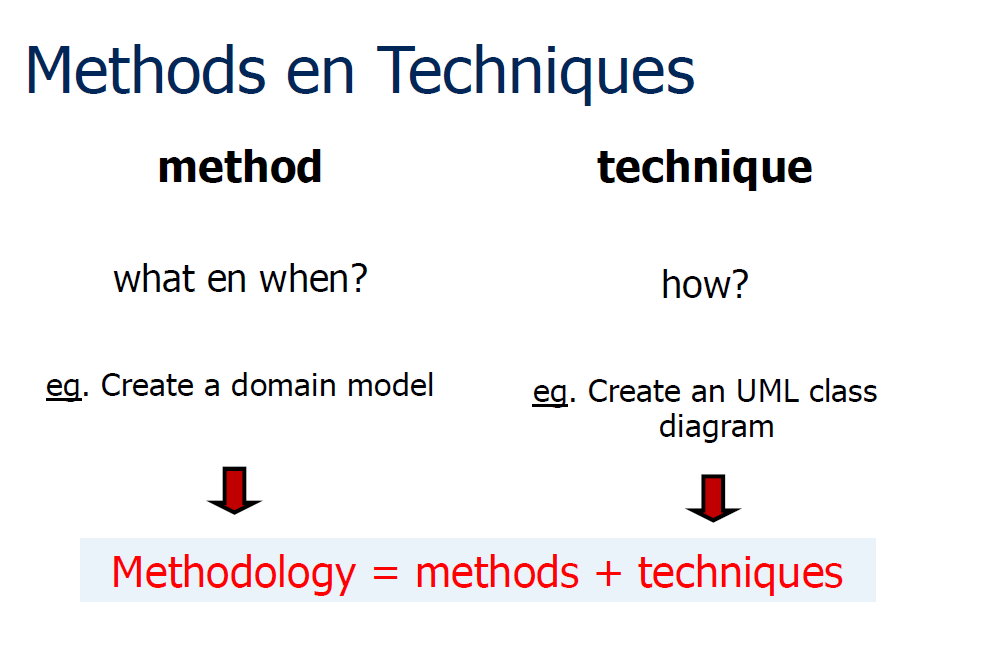
\includegraphics[width=4in]{img/methodstechniques}%
\end{center}



%afbeelding nog plaatsen

\begin{center}
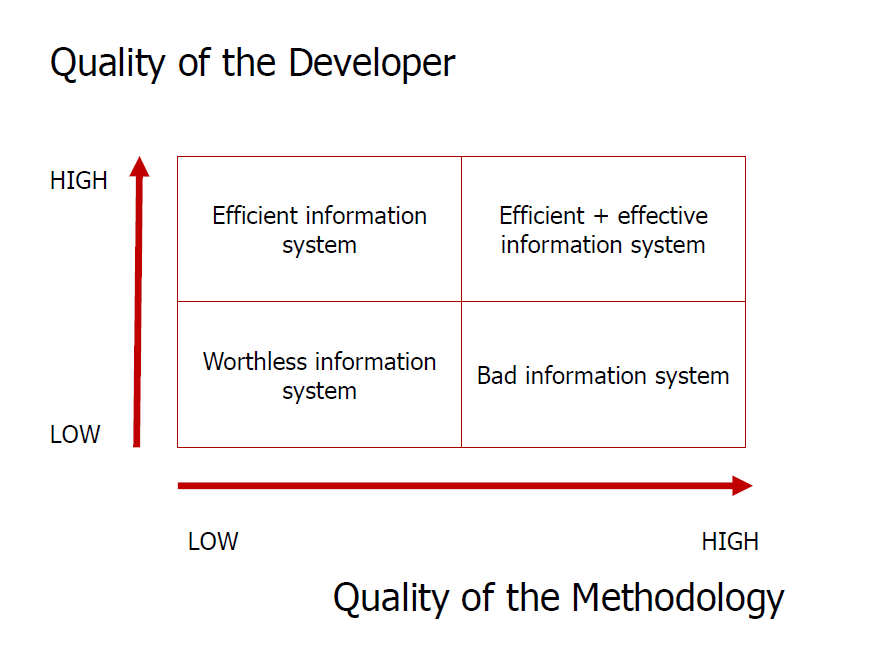
\includegraphics[width=3.6in]{img/quality}%
\end{center}
\newpage
\subsubsection{Rapid Application Development}

Dit is een methodologie waarin de snelheid van ontwikkelen benadrukt wordt, door het heel uitgebreid betrekken van de business professional in de snelle, iteratieve en incrementeel opgebouwde prototypes. Hierbij worden bij elke iteratie nieuwe functionaliteiten toegevoegd aan de op te leveren oplossing, tot uiteindelijk het systeem volledig afgewerkt opgeleverd kan worden.
Vanaf de publicatie door een groep softwareontwikkelaars van het Manifesto for Agile Software Development1 in 2001 wordt voor deze vorm van systeemontwikkeling in het algemeen de term \textbf{agile} gebruikt.

Gedurende de laatste twintig jaar zijn de agile methoden meer en meer dominant geworden. In de jaren negentig ging de meeste aandacht uit naar wat Rapid Application Development (RAD) genoemd werd.

Volgens het manifest kent agile-systeemontwikkeling twaalf grondbeginselen:

\begin{enumerate}
    \item Klanttevredenheid (snelle oplevering van werkende software).
    \item Accepteren dat gebruikerseisen en -wensen veranderen, ook later in het project.
    \item Werkende software wordt regelmatig opgeleverd (liever in weken dan in maanden).
    \item Werkende software is het belangrijkste meetpunt voor het bepalen van de voortgang.
    \item Duurzame systeemontwikkeling.
    \item Nauwe, dagelijkse samenwerking tussen klanten/gebruikers en ontwikkelaars.
    \item Face-to-face communicatie heeft de sterke voorkeur (hele team in dezelfde ruimte).
    \item Projecten worden opgezet rond gemotiveerde individuen die je kunt vertrouwen.
    \item Voortdurende aandacht voor technische excellence en goed ontwerp.
    \item Eenvoud (de kunst om de hoeveelheid werk die niét wordt gedaan te maximaliseren) is essentieel.
    \item Zelf-organiserende teams.
    \item Voortdurende aanpassing aan veranderende omstandigheden.
\end{enumerate}
\newpage
Termen die hier veel gehanteerd worden zijn:

\begin{itemize}
    \item \textbf{Time-box.}
\textcolor{red}{Tijdsperiode die op voorhand bepaald wordt en op basis waarvan uitbreidingen opgeleverd worden.}
    \item \textbf{Iteratie}.
\textcolor{red}{Een iteratieve benadering van systeemontwikkeling betekent niet meer dan dat de resultaten van een of meer activiteiten worden teruggekoppeld, besproken en eventueel aangepast.}
    \item \textbf{Incrementele systeemontwikkeling.}
\textcolor{red}{Het stap voor stap ontwikkelen van informatiesystemen, waarbij elke stap een werkend en bruikbaar - klein of groot - deelsysteem oplevert dat wordt toegevoegd aan hetgeen in eerdere stappen is opgeleverd}. Hierbij moet eerst bepaald worden welke stappen of bouwstenen in het gewenste informatiesysteem te onderkennen zijn. Een increment is vervolgens de stap die nodig is voor analyse, ontwerp, realisatie en invoering van een bouwsteen. Alle incrementen, na de eerste, profiteren van wat in het voorafgaande geleerd is. Een increment wordt ontwikkeld in een zogenaamde time-box. Over de wenselijke doorlooptijd van zo'n time box verschillen de meningen nogal. Sommigen vinden drie tot negen maanden acceptabel, terwijl anderen één tot vier weken ook voldoende vinden.
    \item \textbf{Sprint, Iteratie.}
\textcolor{red}{Ontwikkeling die gebeurt tijdens het verloop van de time-box en waarbinnen nieuwe functionaliteiten toegevoegd worden.}
    \item \textbf{User story.}
\textbf{Functionaliteit die door de klant gevraagd wordt.}
    \item \textbf{Backlog}.
\textcolor{red}{De volledige lijst van user stories die ontwikkeld moeten worden}
    \item \textbf{Retrospective}.
Na afloop van de iteratie wordt een feedback sessie georganiseerd waarbinnen de lessons-learned opgesomd worden.
\item \textbf{Scrum}.
Raamwerk voor agile management van softwareontwikkeling en meer een projectmanagementmethode dan een methode waarin concrete tools en technieken worden aangeboden om software mee te ontwikkelen.
\end{itemize}

\newpage
%7.
\subsection{Benaderingswijzen}

Bij het ontwerpen van een informatiesysteem kan vanuit verschillende zichtpunten gewerkt worden. Een aantal van die benaderingswijzen worden hieronder beschreven.

\subsubsection{de neem-waar benadering}

In deze benadering wordt vertrokken vanuit het bestaande systeem, dat eerst grondig onderzocht wordt. Daartoe is het noodzakelijk eerst het huidige systeem te modelleren.

Dit omwille van een aantal redenen :

\begin{itemize}
    \item Het is meestal eenvoudiger om te beginnen met het modelleren van iets dat al bestaat, dan om iets te modelleren wat nog niet bestaat en daardoor heel abstract is.
    \item Het huidige systeem kan gemodelleerd worden om na te gaan of er in de loop van de tijd bedrijfsfuncties veranderd of zelfs weggelaten zijn ten opzicht van de vereisten voor het nieuwe systeem.
    \item Voor en na figuren van het huidige en het toekomstige systeem kunnen gemaakt worden om deze met elkaar te kunnen vergelijken en aldus voor en tegen van het gewenste systeem te kunnen evalueren.
    \item Het model van het huidige systeem kan nuttig zijn om de gegevensconversie van oud naar nieuw voor te bereiden.
\end{itemize}

\subsubsection{De neem-afstand benadering}

Bij deze benadering wordt afstand genomen van het huidige systeem. Er wordt dus vertrokken vanaf nul, zonder rekening te houden met de huidige situatie. Er zijn een aantal redenen om volgens deze benadering te werken.

Voorbeeld. Het huidige systeem voldoet helemaal niet meer en men wil een volledige vernieuwing.

\subsubsection{De gegevensgerichte benadering}

Bij deze benadering wordt het ganse systeem gemodelleerd vanuit de gegevens. M.a.w. eerst wordt een gegevensmodel opgebouwd en dan wordt de rest van het systeem daar rond gebouwd.

\subsubsection{De procesgerichte benadering}

Bij deze benadering wordt het systeem gemodelleerd vanuit de processen. M.a.w. eerst wordt een procesmodel gebouwd dat de functionaliteiten van het systeem voorstelt en dan wordt daaruit de rest van het systeem gebouwd.

\subsubsection{De communicatiebenadering}

Bij deze benadering gaat men uit van de communicatiemogelijkheden die voor de business professionals voorzien worden dank zij het informatiesysteem. Het gaat hier dus met andere woorden over het conceptueel model van het informatiesysteem. Een techniek die hiervan uitstekend geschikt is, is INHAM (Nijssens Analyse Methode).

\subsection{Project management vs. proces management}

Proces management is een activiteit die documenten beheert, de gekozen methodologie ondersteunt en verbetert. Het gaat over de fasen die doorlopen worden, de stappen die binnen die fasen uitgevoerd moeten worden, de mijlpaalproducten die gecreëerd moeten worden en de kwaliteitsstandaarden die consistent toegepast moeten worden bij alle projecten.

Project management is het proces van afbakenen, plannen, organiseren, en controleren van een project om een informatiesysteem te ontwikkelen tegen minimale kost, binnen een vooraf gespecificeerde tijdsspanne en tegen een aanvaardbare kwaliteit.

Hier zijn een aantal termen wel heel belangrijk:

\begin{itemize}
    \item Probleemomschrijving:
    
in deze beschrijving worden de problemen in de huidige situatie beschreven, en gecategoriseerd. Er worden richtlijnen gegeven van hoe het toekomstige systeem er moet uitzien, wat de systeemeisen zijn, wat de beperkingen zijn waarmee rekening gehouden moet worden en wat de visie is voor de oplossing.
    \item Constraint:
    
elke factor, beperking, bedenking die een oplossing van het probleem zou kunnen beperken.
    \item Project plan (Service-level agreement - SLA):
    
contract met het management en de business professional om het informatiesysteem te ontwikkelen of uit te breiden, waarin de visie, het bereik, de user-requirements (hoog niveau - gewenste functionaliteiten), de beperkingen, de planning en het budget beschreven worden.
\item Request for proposal (RFP):

Een formeel document dat alle business, technische en onderhouds- requirements voor een te ontwikkelen applicatie beschrijft. Dit document wordt naar mogelijke leveranciers verstuurd. Zij kunnen dan een voorstel opmaken waarin beschreven wordt hoe zij een applicatie kunnen ontwikkelen en wat de kostprijs zal zijn. Deze beschrijving wordt dan de \textbf{bid-offering} genoemd.
\item Gap analysis:

Een vergelijking van business en technische systeemeisen voor een commerciële applicatie met de mogelijkheden en eigenschappen van een specifieke commerciële applicatie met als doel het aanduiden van de eisen die niet gehaald kunnen worden.
\end{itemize}
\newpage
Binnen software ontwikkeling, wordt regelmatig verwezen naar het \textbf{PIECES} framework:

\begin{center}
\noindent\fbox{%
    \parbox{\textwidth}{%
P performantie verbeteren\newline
I Informatie ( en gegevens) verbeteren\newline
E Economie verbeteren, kosten controleren en/of verhogen van de winst\newline
C Controle en veiligheid verbeteren\newline
E Efficiëntie van mensen en processen verbeteren\newline
S Service naar klanten, leveranciers, partners, werknemers, enz verbeteren
    }
}
\end{center}

PIECES is een heel bruikbare, nuttige manier om problemen te karakteriseren en te beschrijven. PIECES kan ook gebruikt worden om systeemeisen (requirements) en oplossingen te beschrijven.